% \chapter{Results}\label{sec:results}

% \section{Ground Truth}{
    
%     As there wasn't a GT for my dataset I considered the very accurate and map based Lio-Sam\footnote{LIO-SAM: Tightly-coupled Lidar Inertial Odometry via Smoothing and Mapping \citep{liosam2020shan}} estimation as the GT for this work. 
    
%     I also considered LOAM\footnote{LiDAR Odometry And Mapping \citep{LOAM}} for another comparison and very importantly as a third and most meaningful alternative I chose the LOAM method without the map procedure as well. This is because my approach is scan based and does not build a map which of course enhances accuracy significantly. So comparing to a scan based method is the only fair comparison.


%     }

% \section{Stepwise Results}{

%     \subsection{Comparison of Separated Components}{
%     \begin{figure}[ht]
%         \centering
%         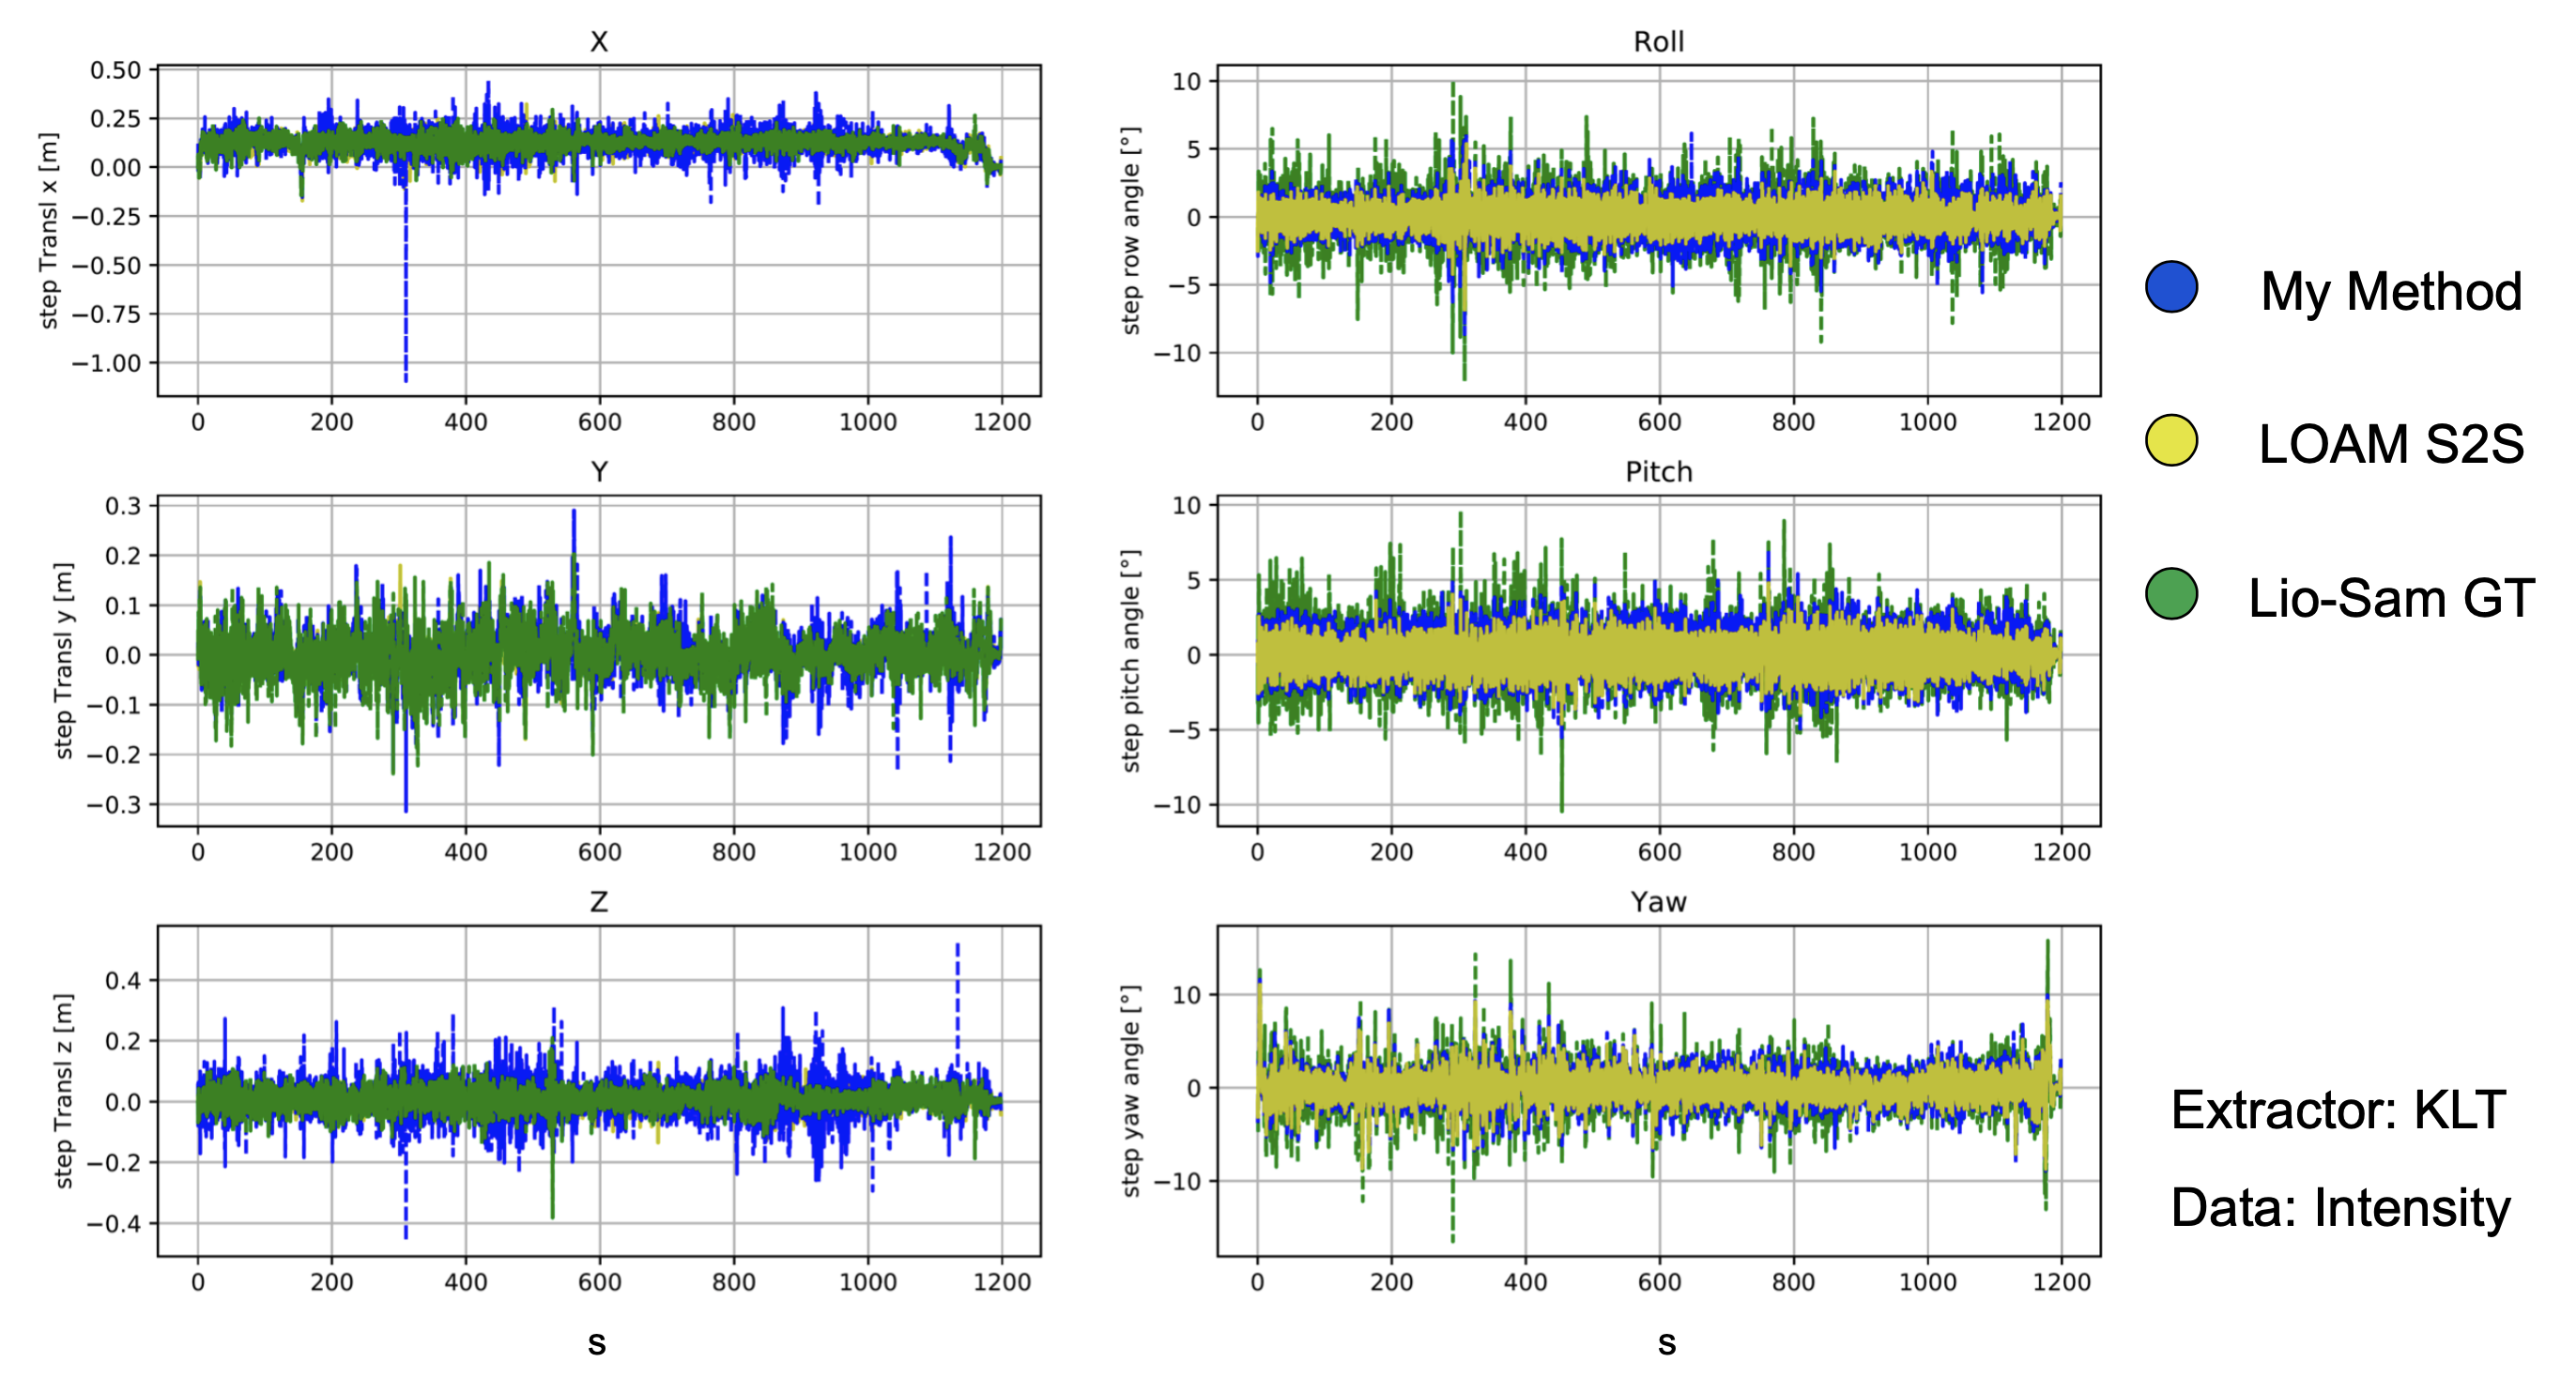
\includegraphics[scale = 0.26]{images/results/steps_klt.png}
%         \caption{Step comparison}
%         \label{fig:step_comparison_klt}
%     \end{figure}

%     In \cref{fig:step_comparison_klt} we can see the step comparison of the three directions as well as the rotation angles. 
    
%     We can also consider the errors at each iteration depicted in the following \cref{fig:step_error_comparison_klt}
%     \begin{figure}[ht]
%         \centering
%         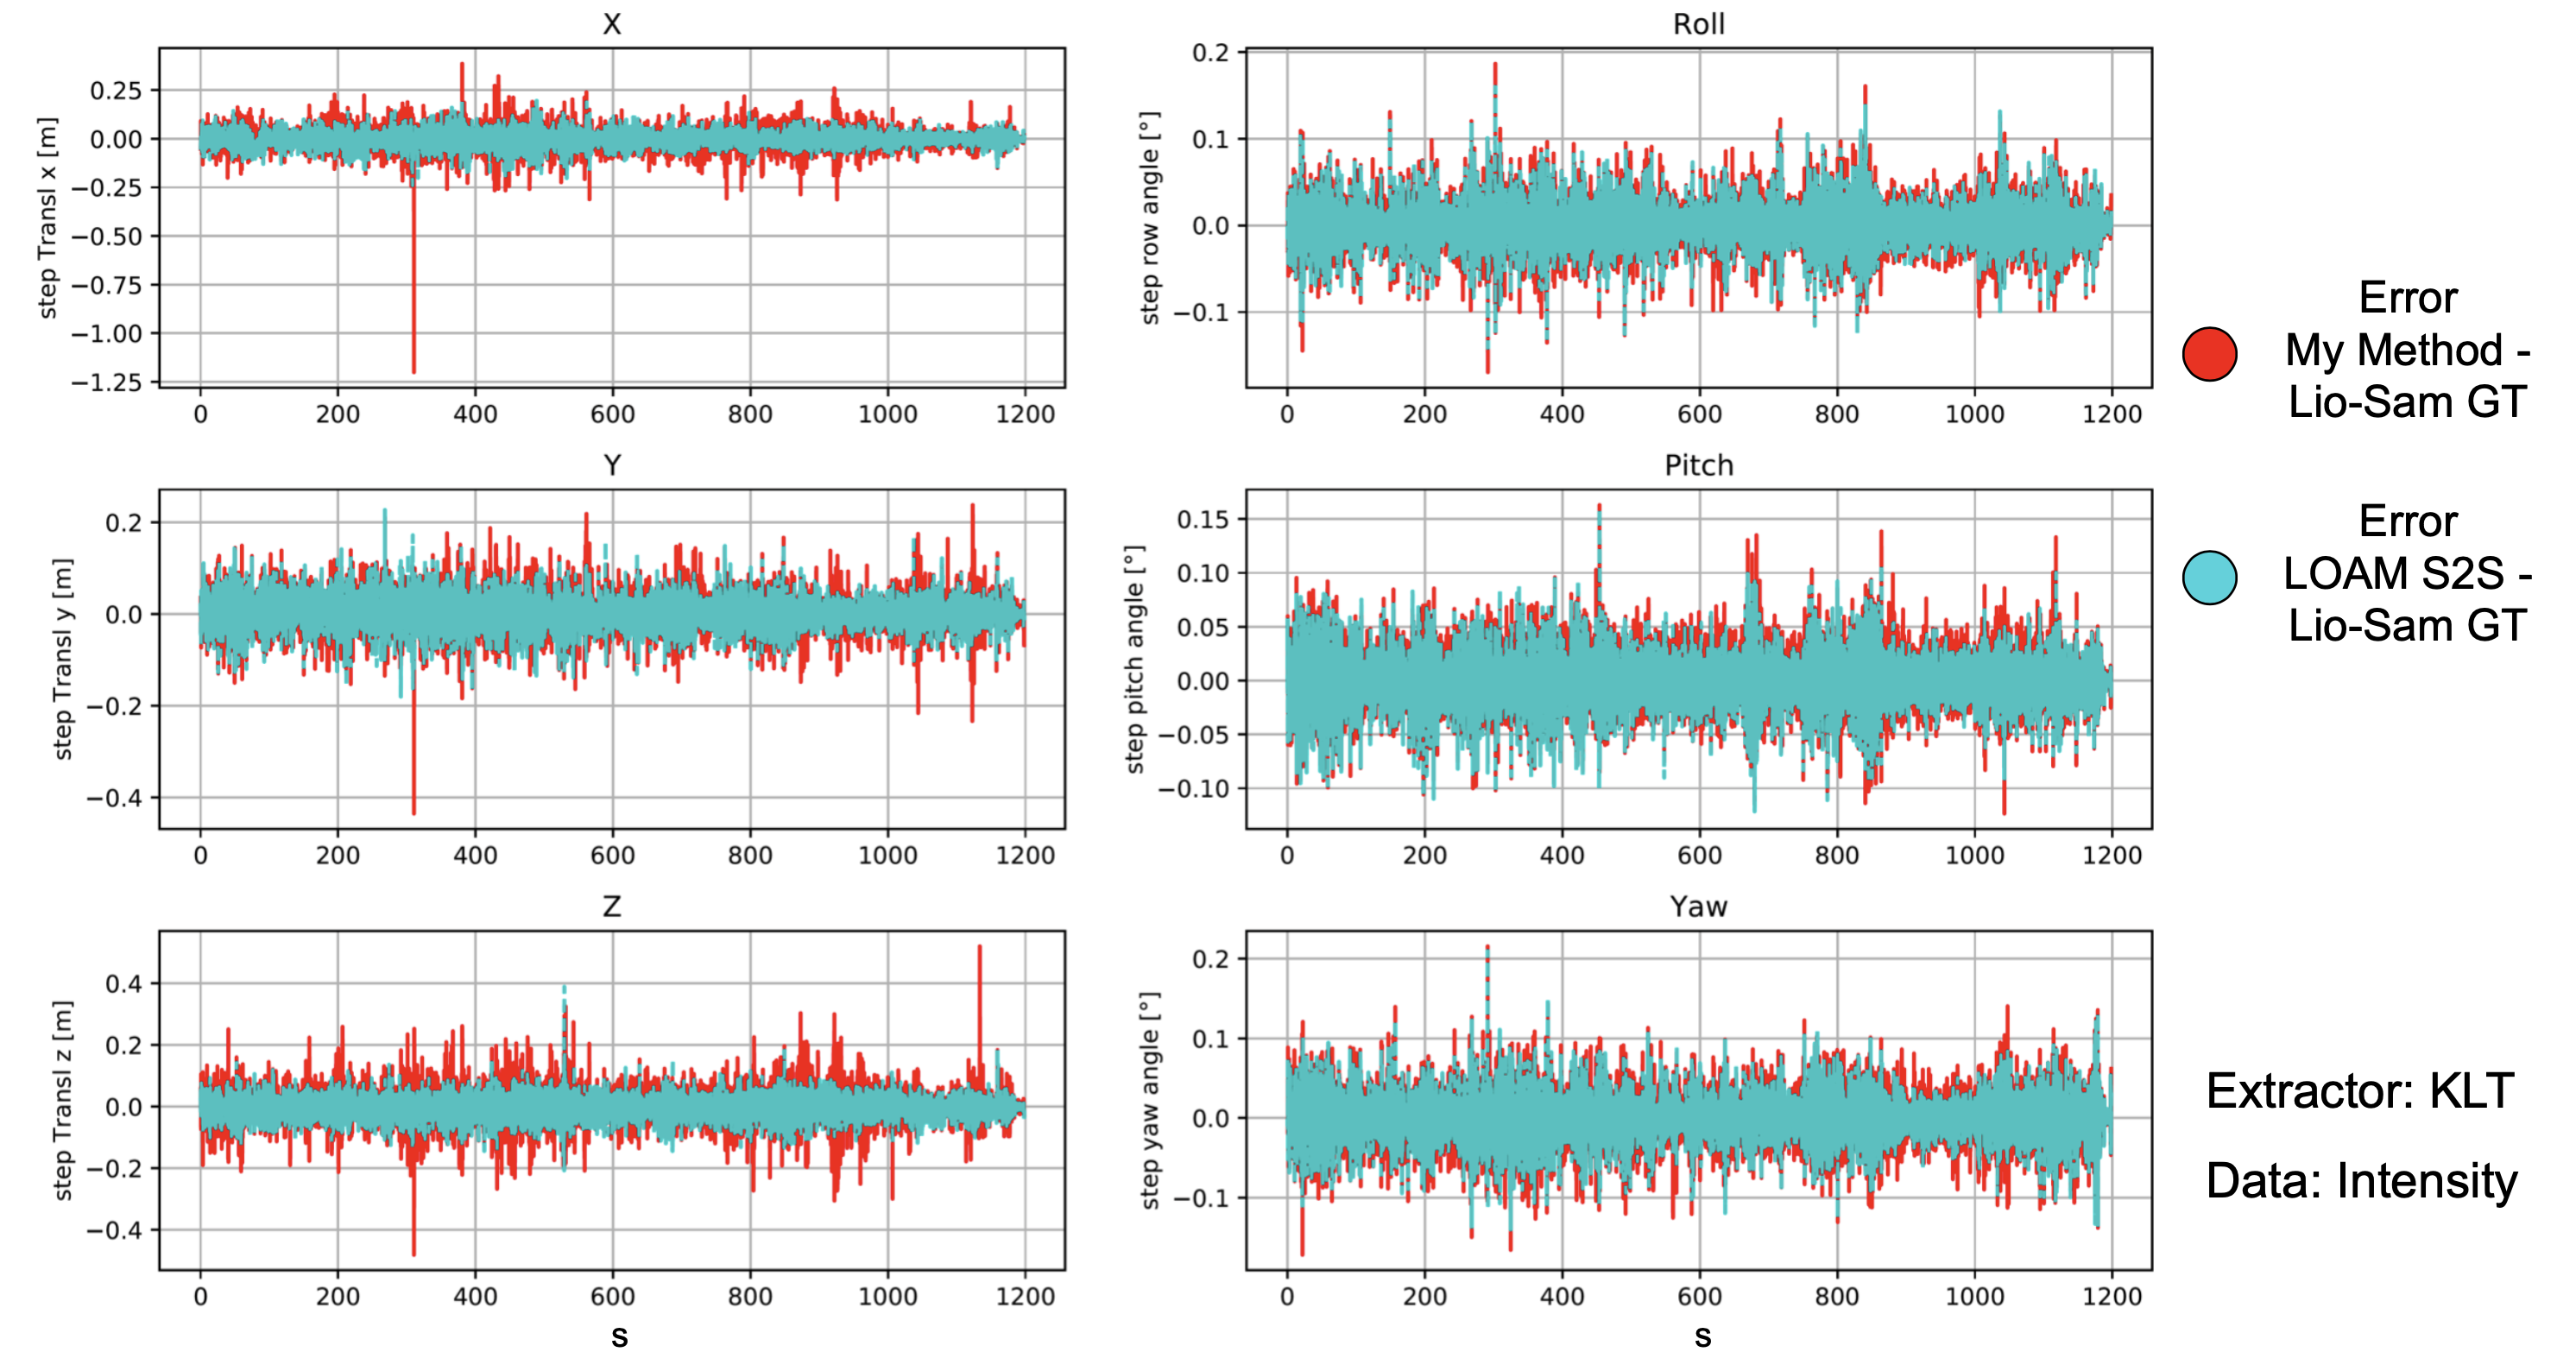
\includegraphics[scale = 0.285]{images/results/step_error_klt.png}
%         \caption{Step Error comparison}
%         \label{fig:step_error_comparison_klt}
%     \end{figure}



%     As we can see in the figures \cref{fig:step_comparison_klt} and \cref{fig:step_error_comparison_klt} there are outliers in the method. However both the step error of this papers method as well as the iterative error of the scan based LOAM method yield values in the same range.

%     }

%     \subsection{Average Step Performance Comparison}{
%     Mean iterative error and standard deviation thereof regarding GT over the whole dataset:

%         \vspace{0.5cm}
        
%         \large
%         \begin{tabular}{p{3cm} p{4.5cm} p{3.5cm} }
%             \textbf{Errors} & \textbf{My Method} & \textbf{LOAM S2S}
%         \end{tabular}

%         \begin{table}[!ht]
%             \setlength{\extrarowheight}{5pt}
%             \centering
%             \large
%             \begin{tabular}{p{2cm} p{2cm} p{2cm} p{2cm} p{2cm} }
%                 \hline
%                  & Mean & STD & Mean & STD\\[12pt]
%                 \hline
%                 X[m] & -0.004 & 0.056 & \text{\color{Green}{-0.002}} & \text{\color{Cyan}{0.035}}\\[3pt]
%                 \hline
%                 Y[m] & \text{\color{Green}{0}} & 0.040 & 0.005 & \text{\color{Cyan}{0.028}}\\[3pt]
%                 \hline
%                 Z[m] & \text{\color{Green}{-0.001}} & 0.058 & -0.004 & \text{\color{Cyan}{0.032}}\\[3pt]
%                 \hline
%                 Roll[°] & \text{\color{Green}{0}} & 0.024 & \text{\color{Green}{0}} & \text{\color{Cyan}{0.021}}\\[3pt]
%                 \hline
%                 Pitch[°] & \text{\color{Green}{0}} & 0.024 & -0.001 & \text{\color{Cyan}{0.020}}\\[3pt]
%                 \hline
%                 Yaw[°] & \text{\color{Green}{0}} & 0.024 & \text{\color{Green}{0}} & \text{\color{Cyan}{0.023}}\\[3pt]
%             \end{tabular}
%             \caption{Average Step Error Comparison}
%             \label{tab:step_errors_klt}
%         \end{table}

%         The data displayed in \cref{tab:step_errors_klt} was achieved using the KLT method on intensity data. Green values are the best achieved mean while light blue indicates the best standard deviation.   

%         When evaluating the numbers we see for my method smaller mean errors on average while LOAM scan 2 scan has smaller deviations from the slightly larger mean error.

        
%     }

% \section{Global Results}{
%     \subsection{Comparison of Separated Components}{

%     Comparing the individual pose components:

%         \begin{figure}[ht]
%             \centering
%             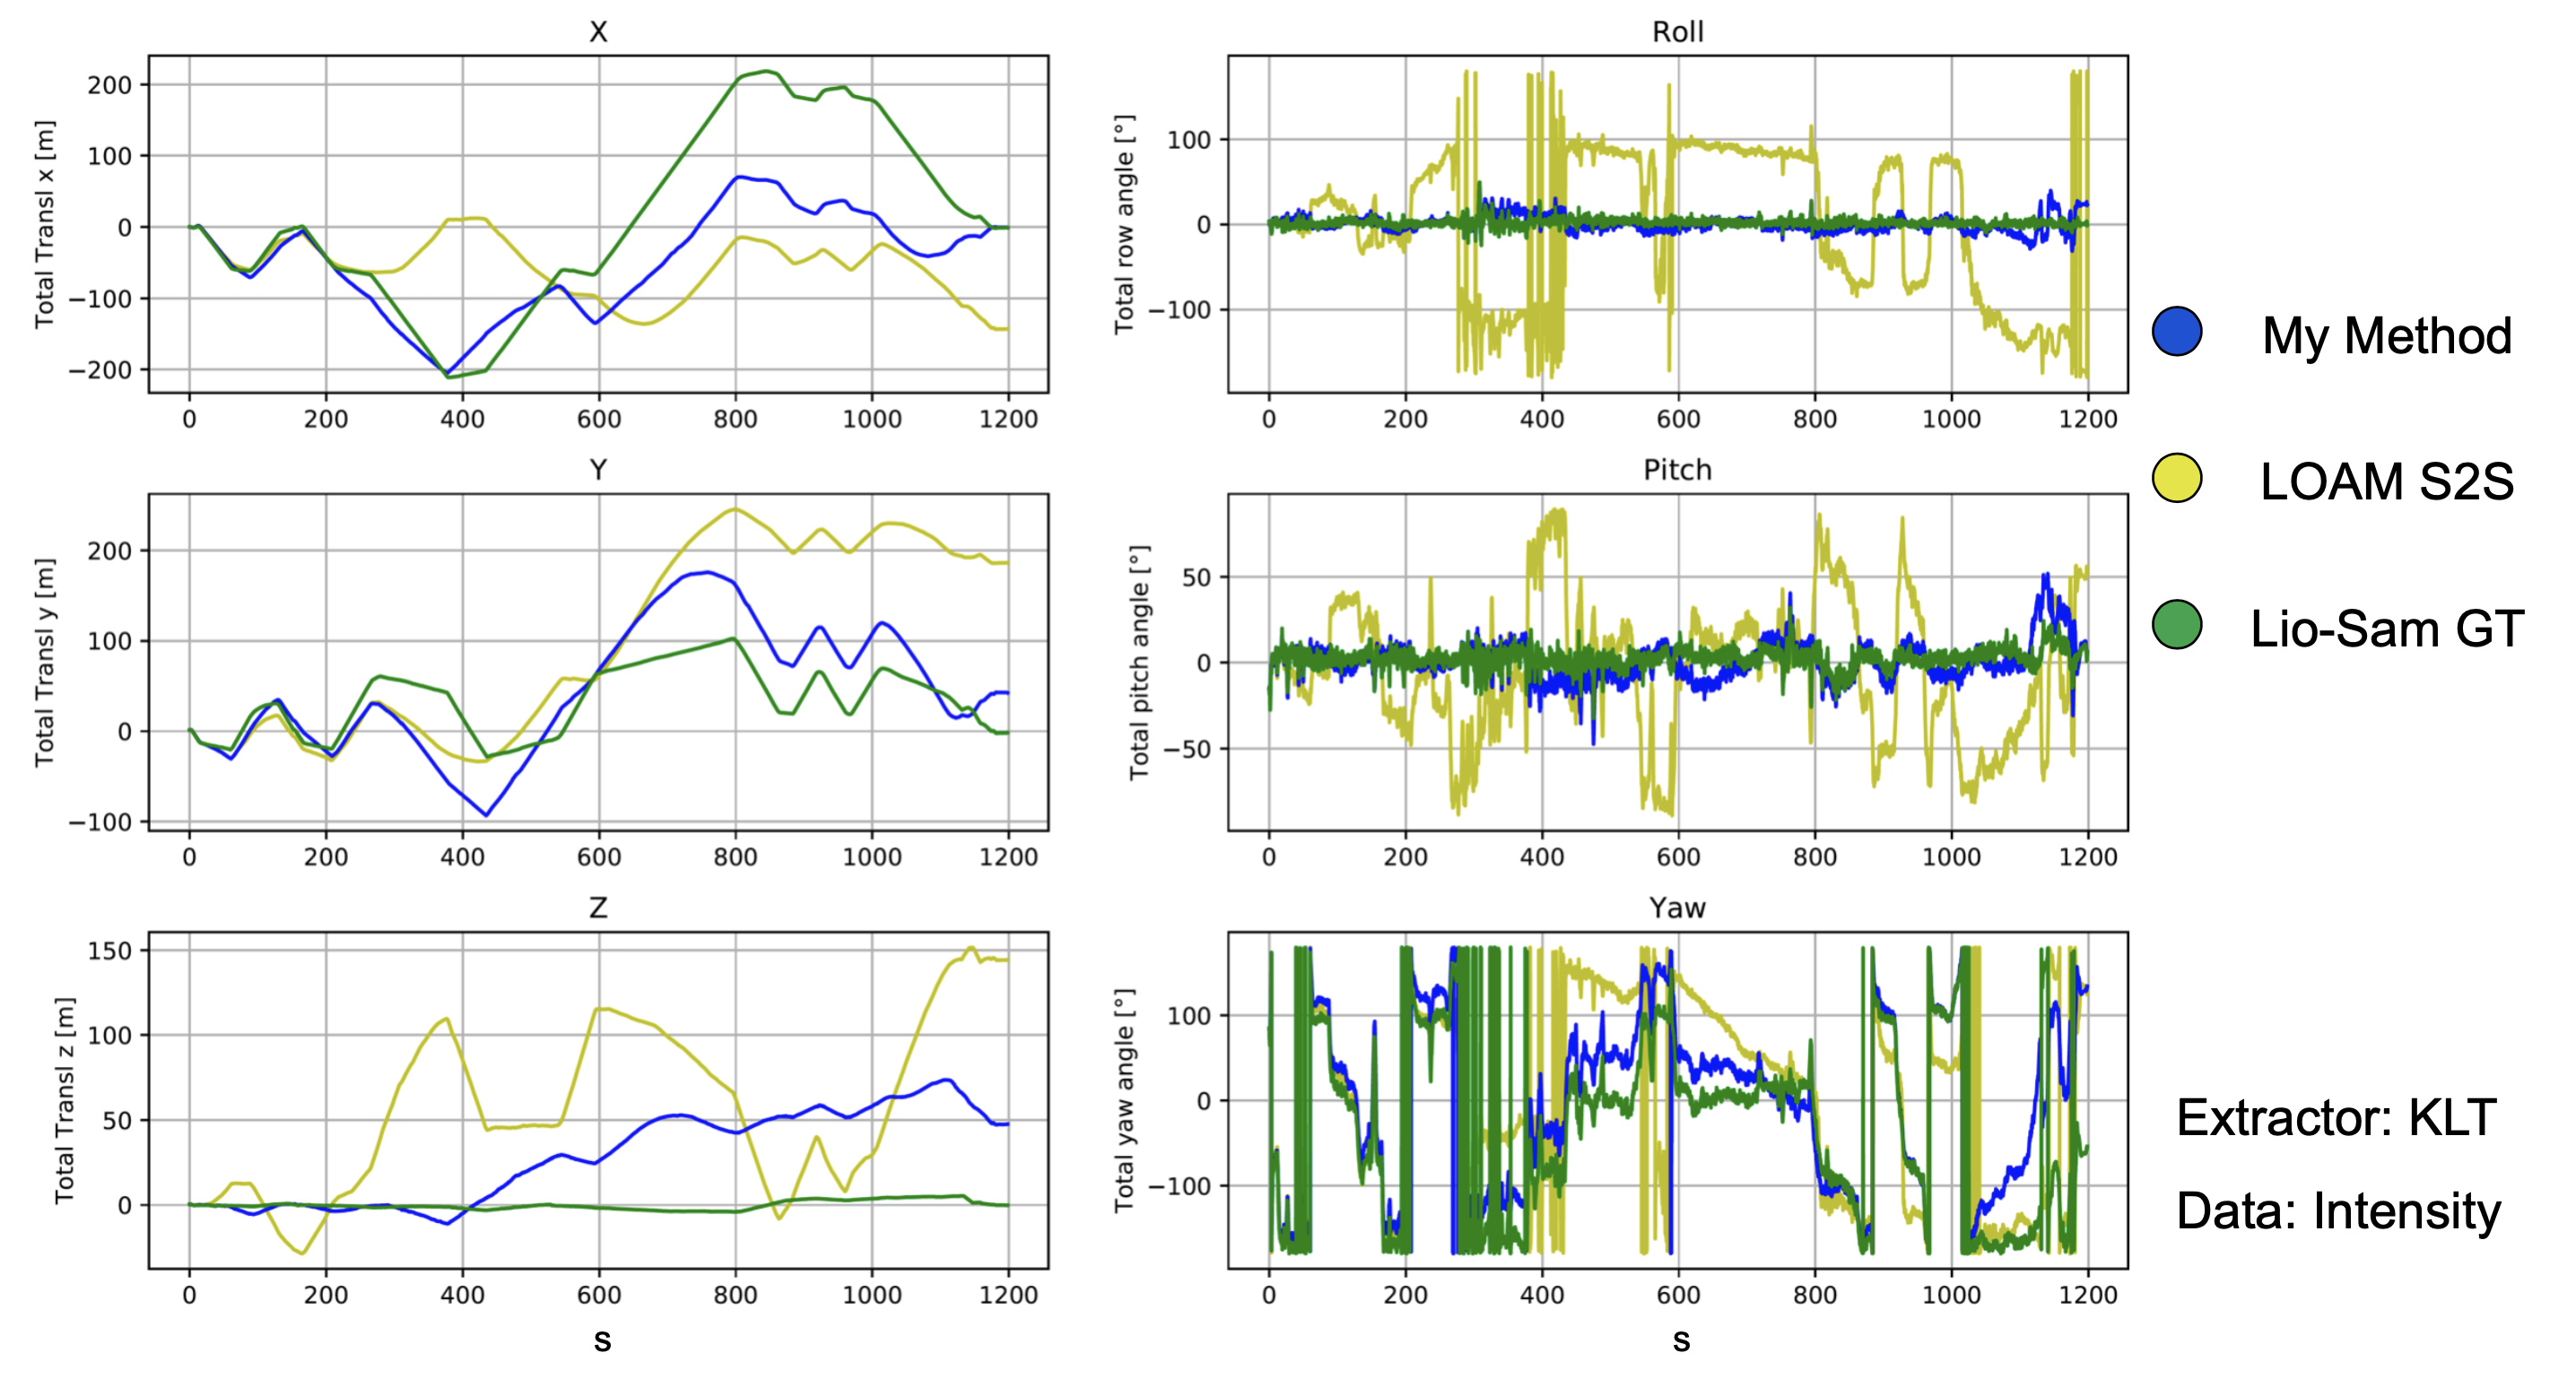
\includegraphics[scale = 0.25]{images/results/pose_klt.png}
%             \caption{Pose comparison}
%             \label{fig:pose_comparison_klt}
%         \end{figure}

%         \begin{figure}[ht]
%             \centering
%             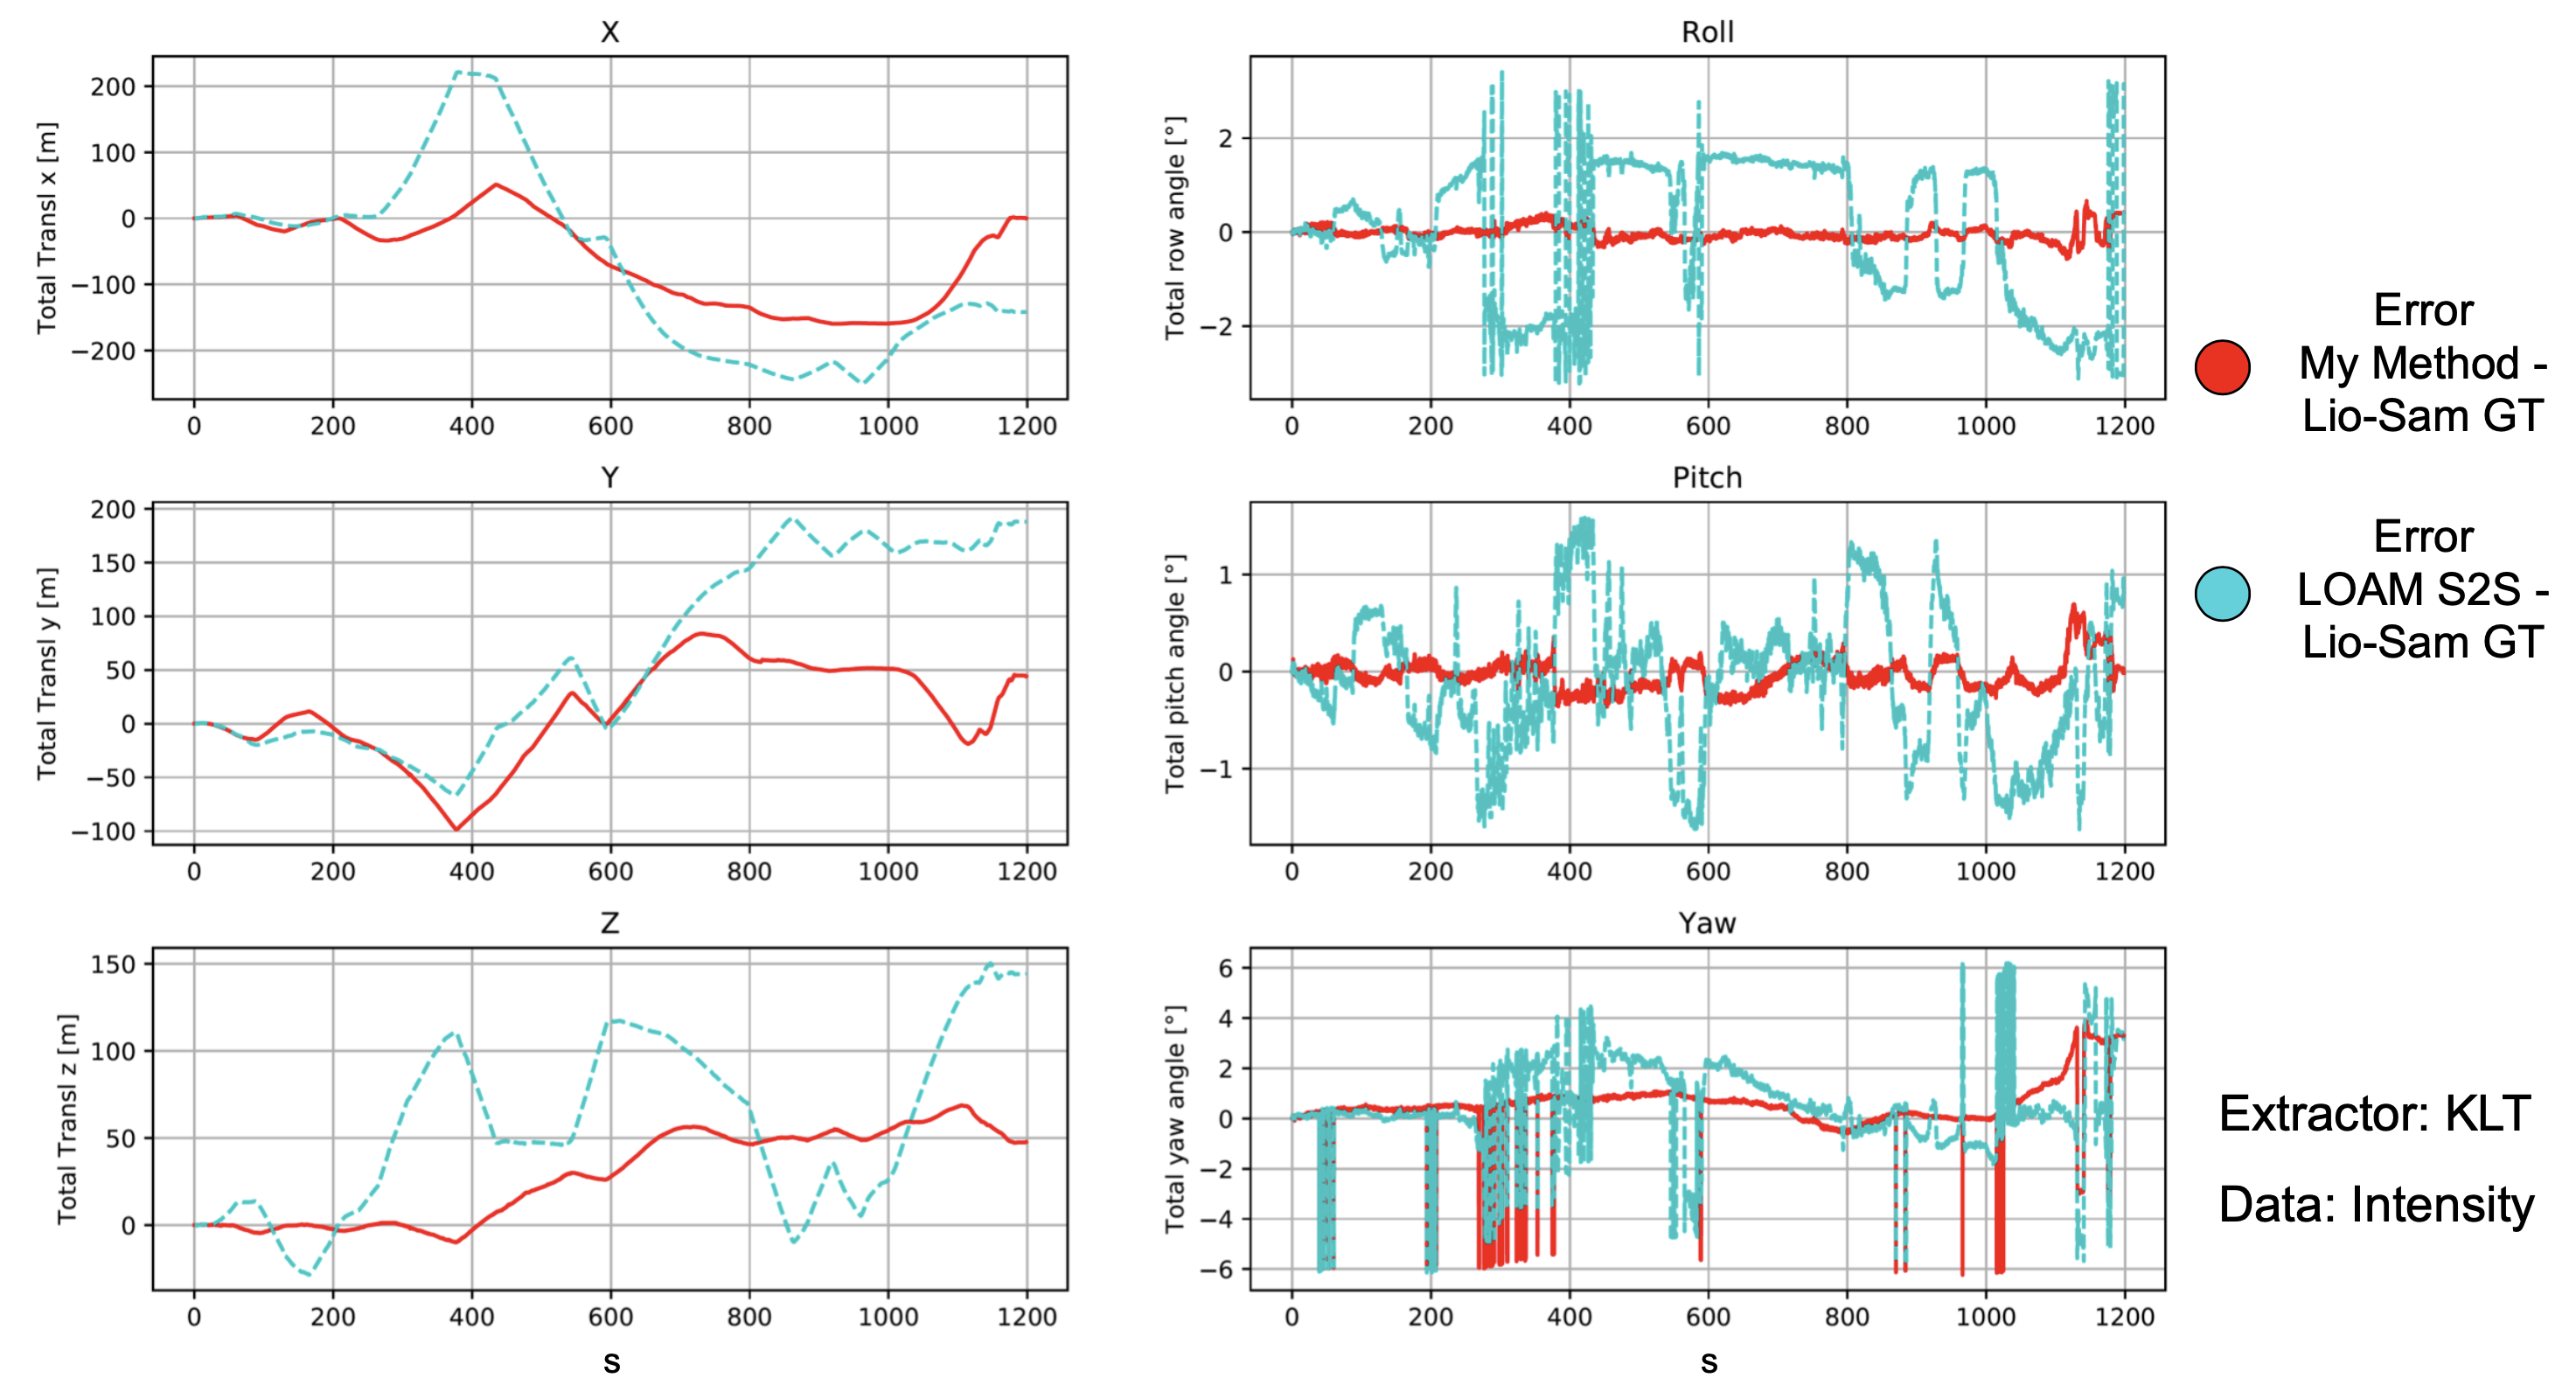
\includegraphics[scale = 0.25]{images/results/pose_error_klt.png}
%             \caption{Pose error comparison}
%             \label{fig:pose_error_comparison_klt}
%         \end{figure}

%         Here in \cref{fig:pose_comparison_klt} and \cref{fig:pose_error_comparison_klt} we can see substantially better global performance of this works method especially regarding the angular development.

%     }

%     \subsection{Comparison of Global Error}{
%         \begin{figure}[ht]
%             \centering
%             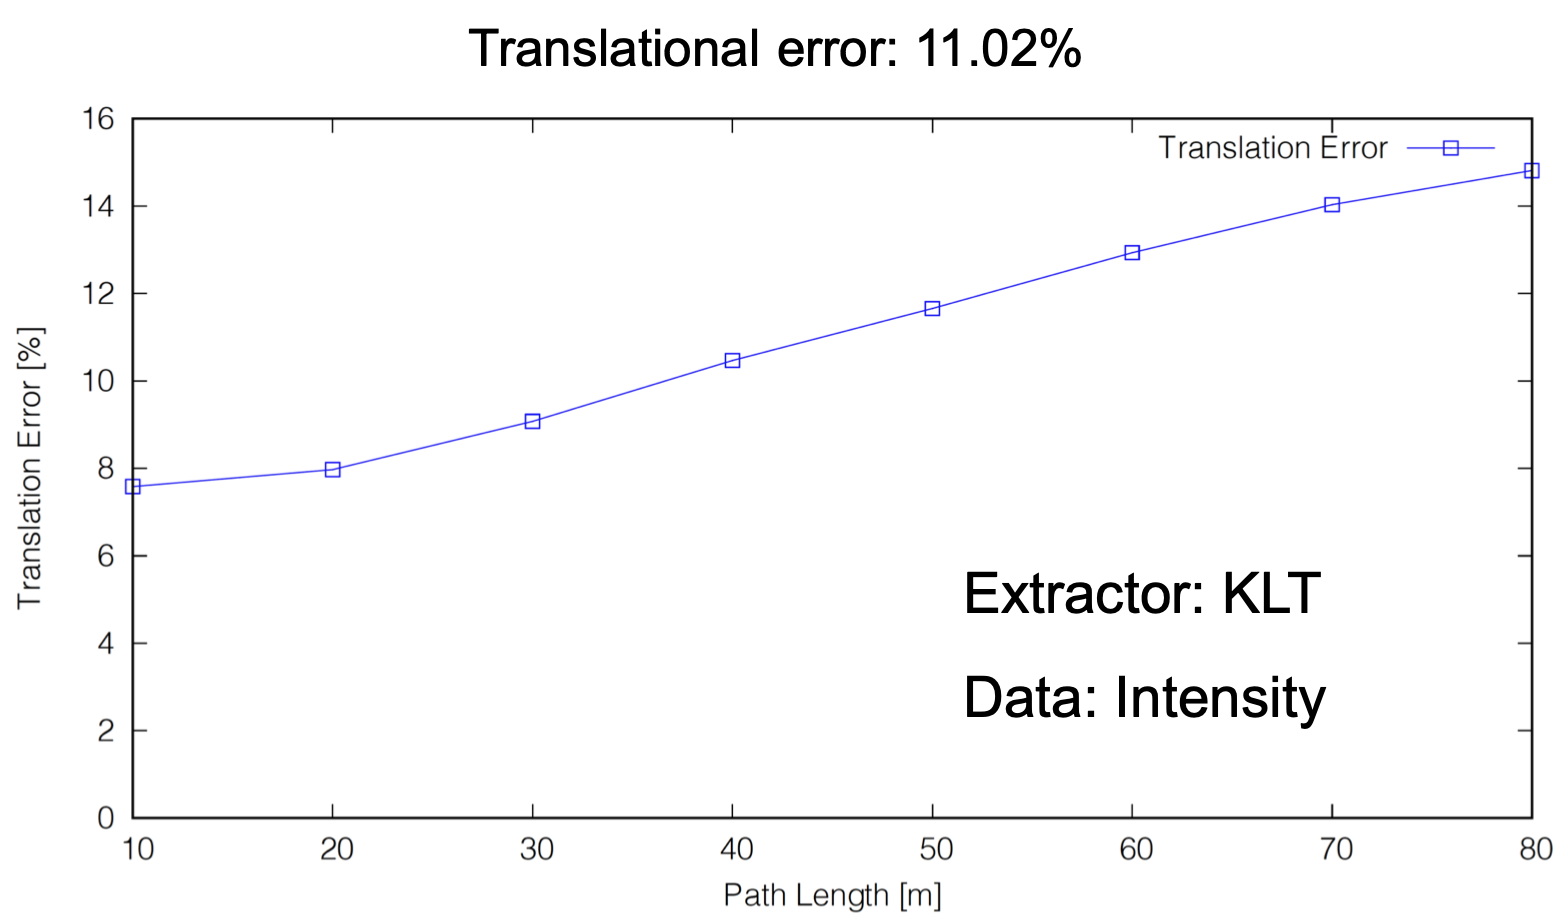
\includegraphics[scale = 0.45]{images/results/mm_drift_translation.png}
%             \caption{My methods translational drift}
%             \label{fig:mm_drift_transl_klt}
%         \end{figure}
        
%         \begin{figure}[ht]
%             \centering
%             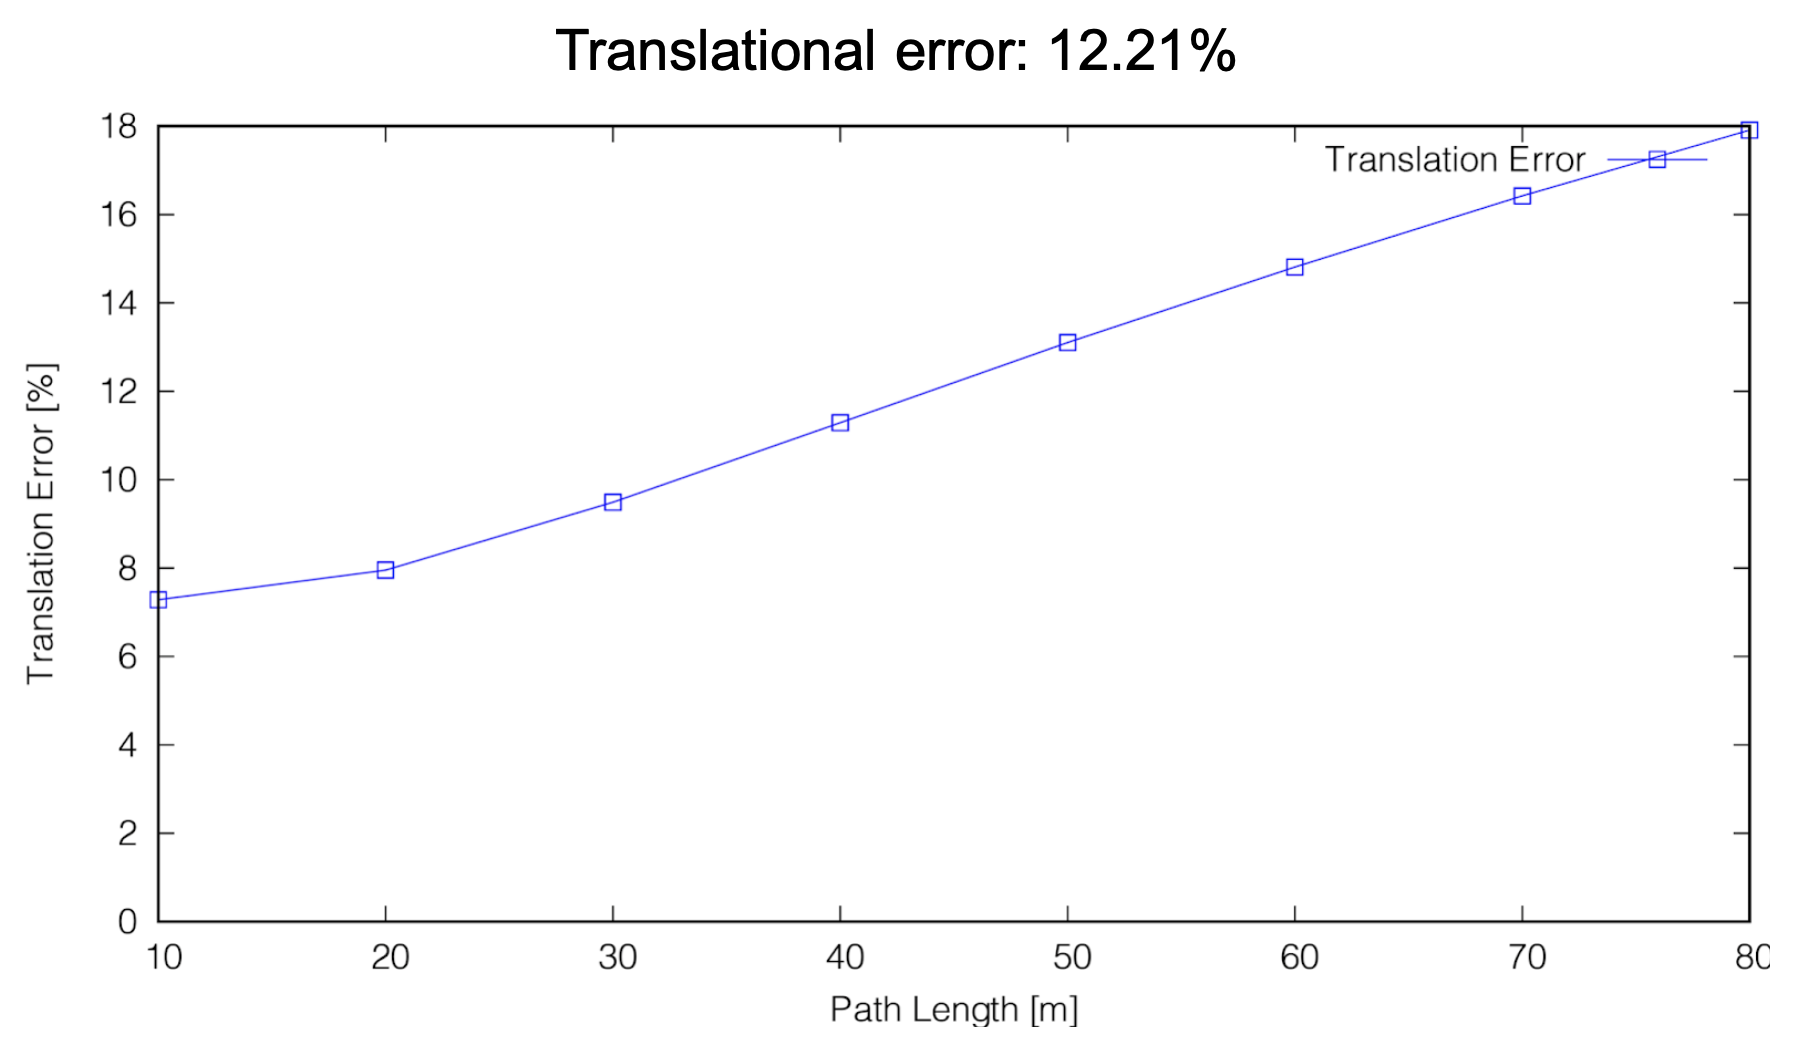
\includegraphics[scale = 0.4]{images/results/loam_drift_transl.png}
%             \caption{LOAM translational drift}
%             \label{fig:loam_drift_transl_klt}
%         \end{figure}
        
%         To account for the drift of the motion estimation a comparison was done after predetermined distance intervals. Here in \cref{fig:mm_drift_transl_klt} to \cref{fig:loam_drift_transl_klt} are the values for the intervals from 10 to 80 meters. It has to be noted that 80 meters is quite a distance and the results from that margin onwards might be slightly deceiving compared to more solid smaller intervals. 
        
%         Averaged over all interval sizes my methods performs a little better as can be seen from the averaged translational error denoted at the top.

%         \clearpage

%         \begin{figure}[ht]
%             \centering
%             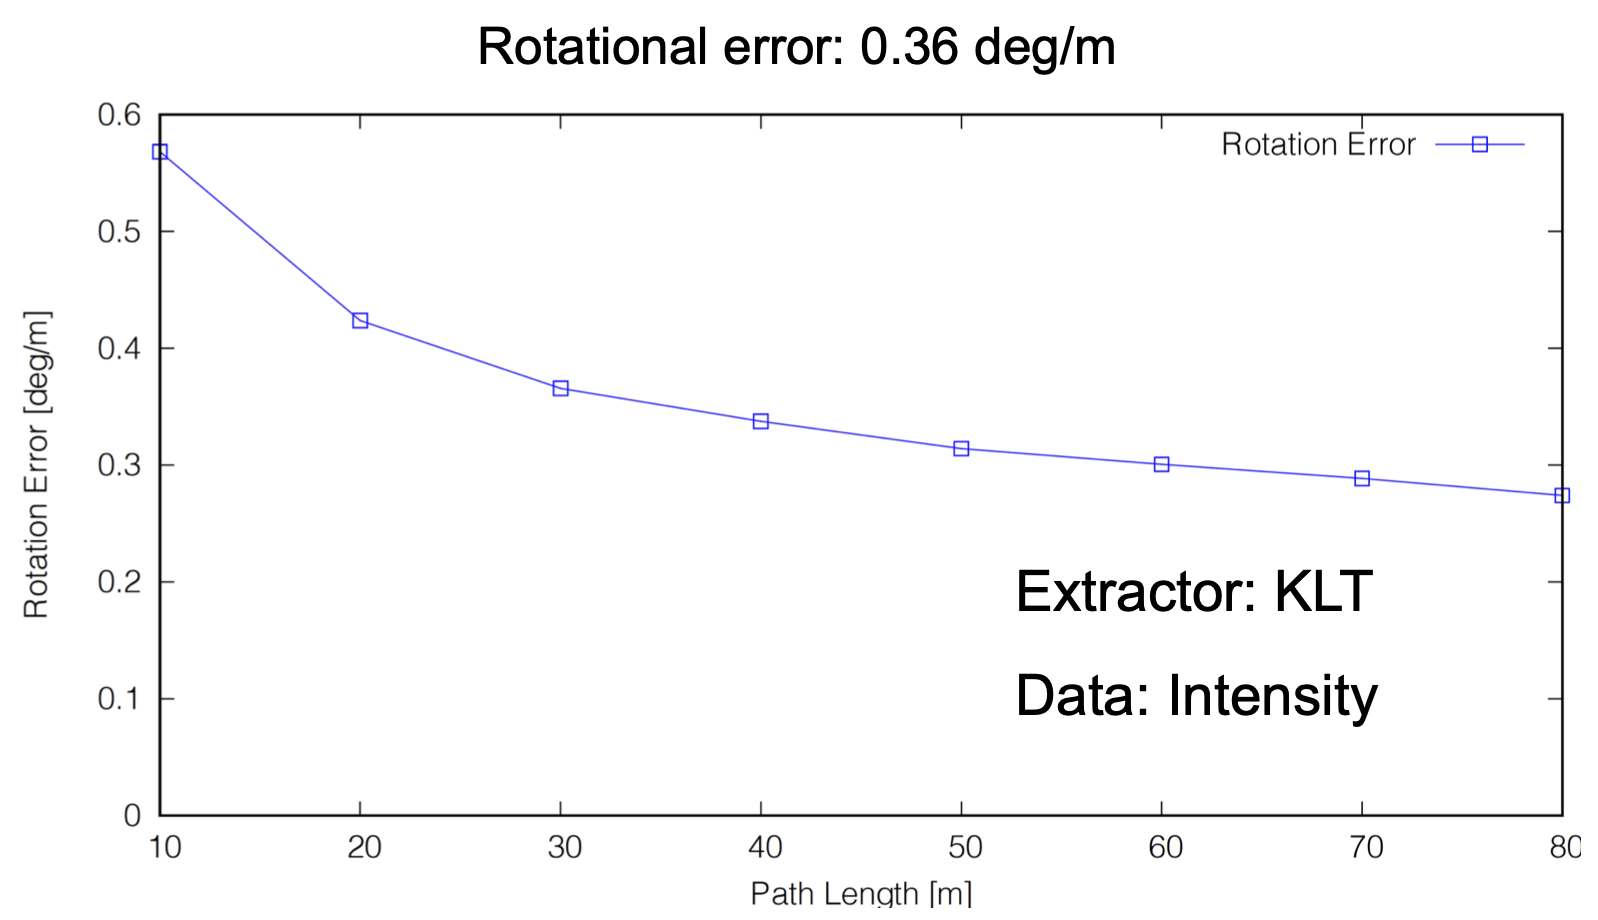
\includegraphics[scale = 0.45]{images/results/mm_drift_angle.png}
%             \caption{My methods angular drift}
%             \label{fig:mm_drift_angle_klt}
%         \end{figure}

%         \begin{figure}[!ht]
%             \centering
%             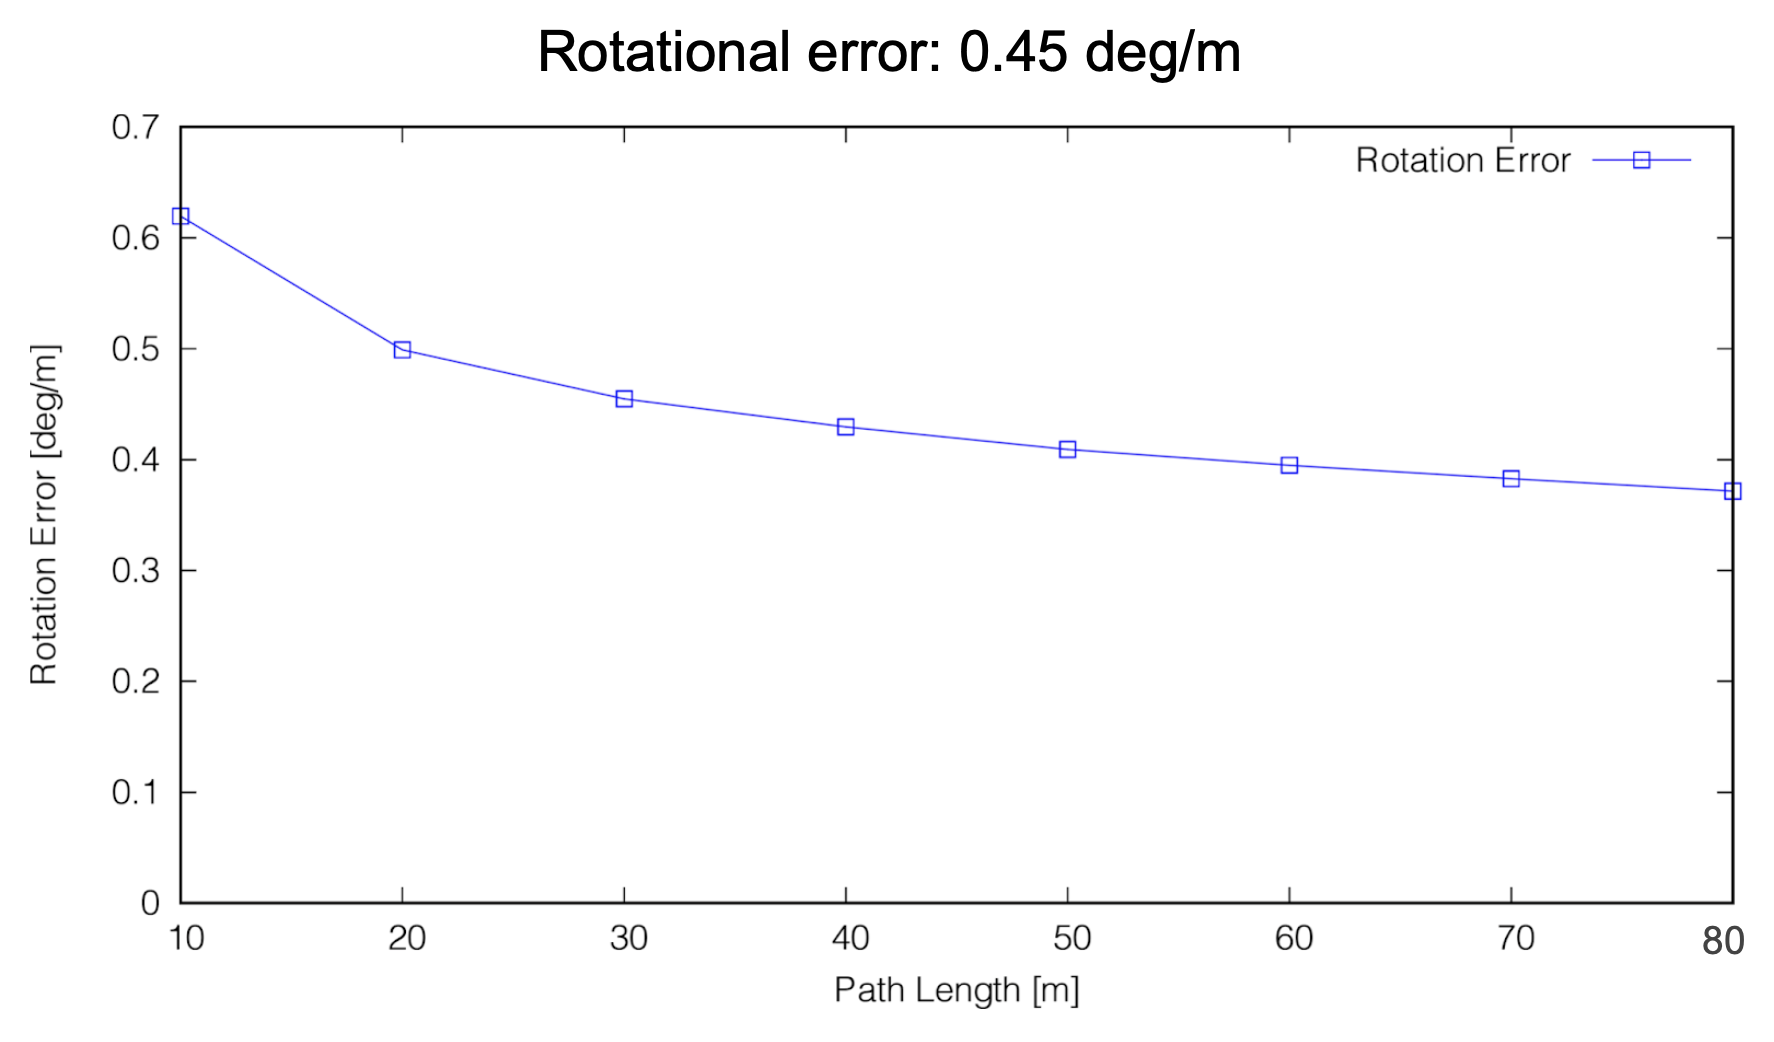
\includegraphics[scale = 0.4]{images/results/loam_drift_angle.png}
%             \caption{loam angular drift}
%             \label{fig:loam_drift_angle_klt}
%         \end{figure}

%         A similar result can be drawn from the angular development. This papers method shows with 0.35 degrees/meter a better performance than the LOAM scan to scan method.
%     }
%     \clearpage

%     \subsection{Comparing Estimated Trajectories}{
%         \begin{figure}[!ht]
%             \centering
%             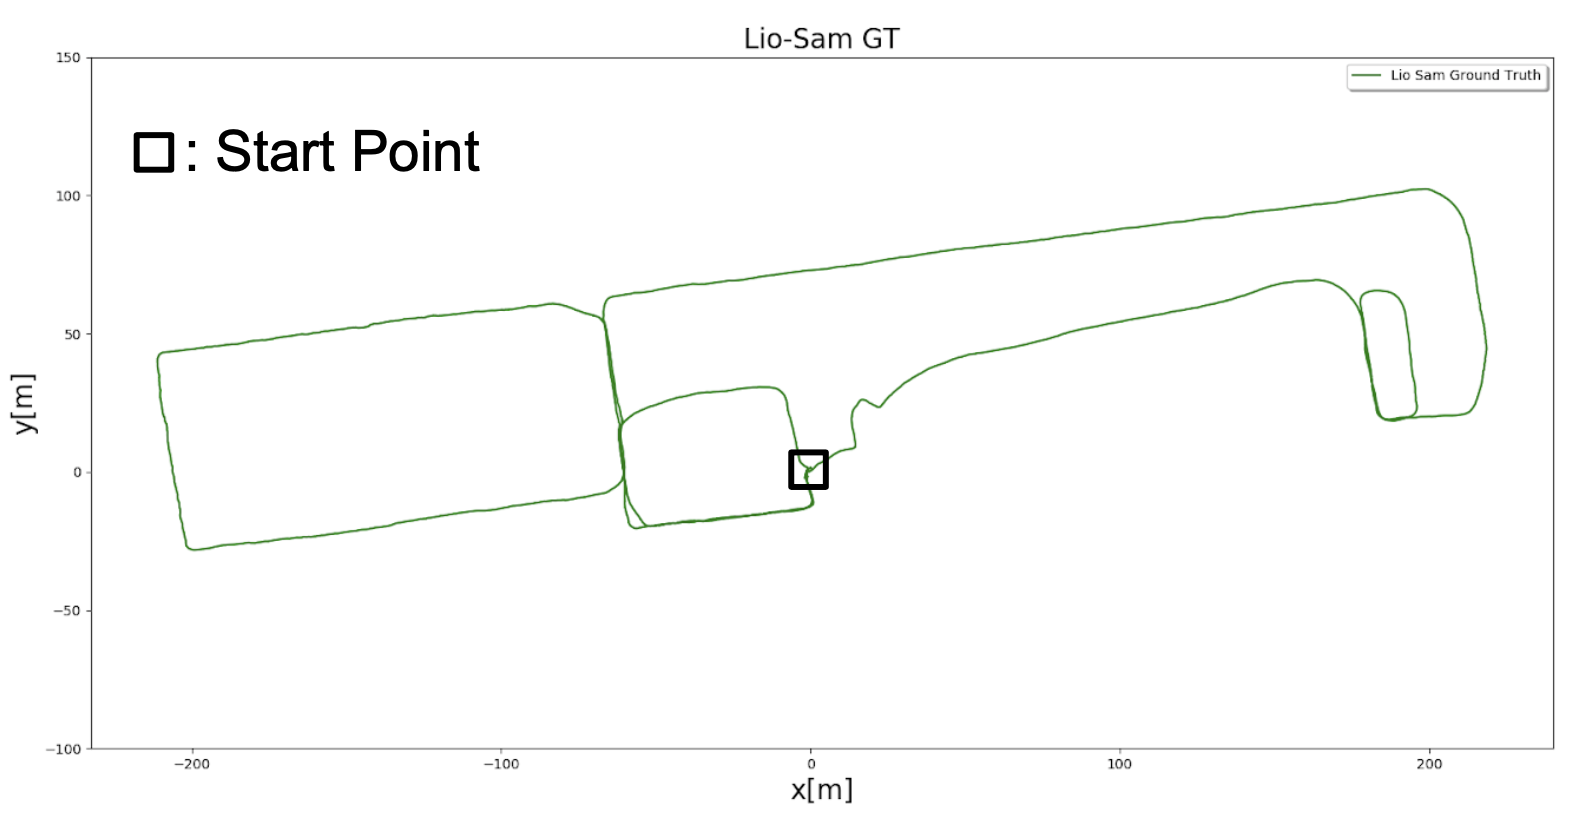
\includegraphics[scale = 0.45]{images/results/GT_trajectory.png}
%             \caption{GT trajectory}
%             \label{fig:GT_trajectory}
%         \end{figure}

%         Indicated on the plot above is the datasets trajectory estimated by Lio-Sam. This will again be considered the ground truth.

%         \begin{figure}[!ht]
%             \centering
%             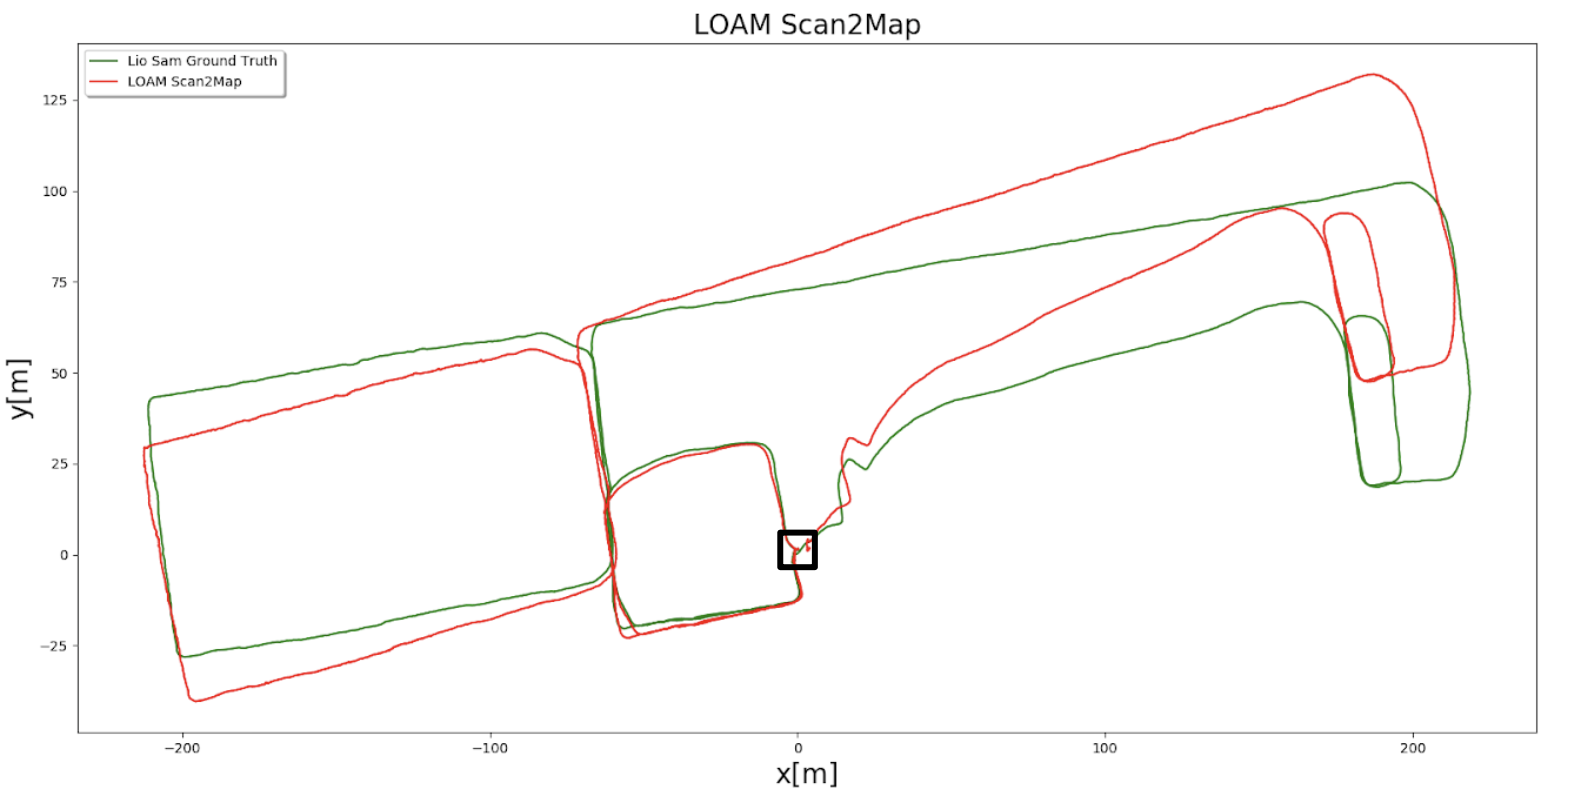
\includegraphics[scale = 0.45]{images/results/loam_s2m_trajectory.png}
%             \caption{LOAM scan to map trajectory}
%             \label{fig:loam_s2m_trajectory}
%         \end{figure}

%         As aforementioned the LOAM method performs very well as it is also map based and thus really accurate.
%         \clearpage

%         \begin{figure}[!ht]
%             \centering
%             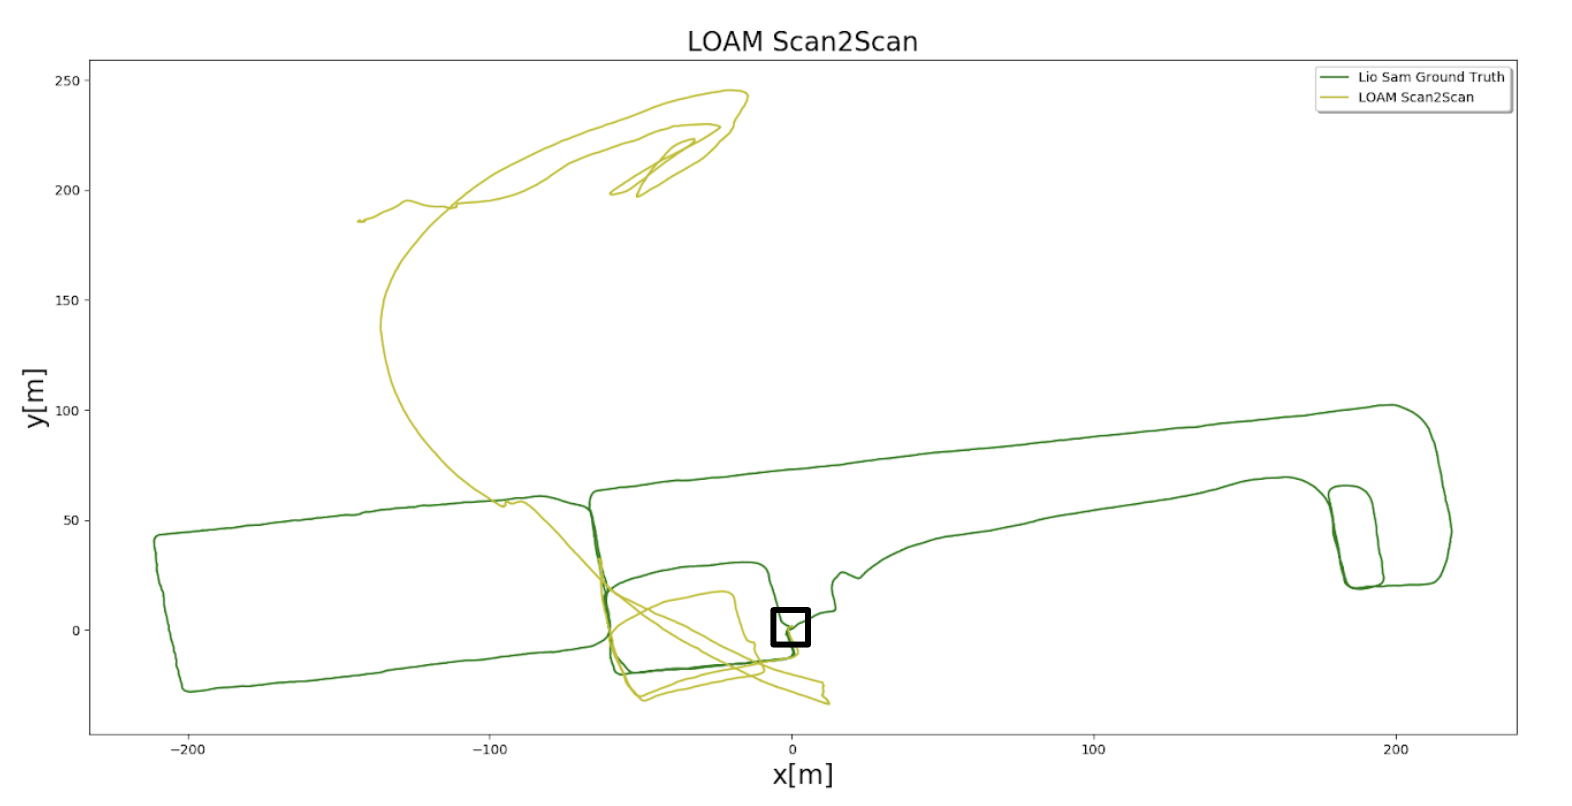
\includegraphics[scale = 0.45]{images/results/loam_s2s_trajectory.png}
%             \caption{LOAM scan to scan trajectory}
%             \label{fig:loam_s2s_trajectory}
%         \end{figure}

%         Considering the solely scan based LOAM estimation it looks quite poor.

%         \begin{figure}[!ht]
%             \centering
%             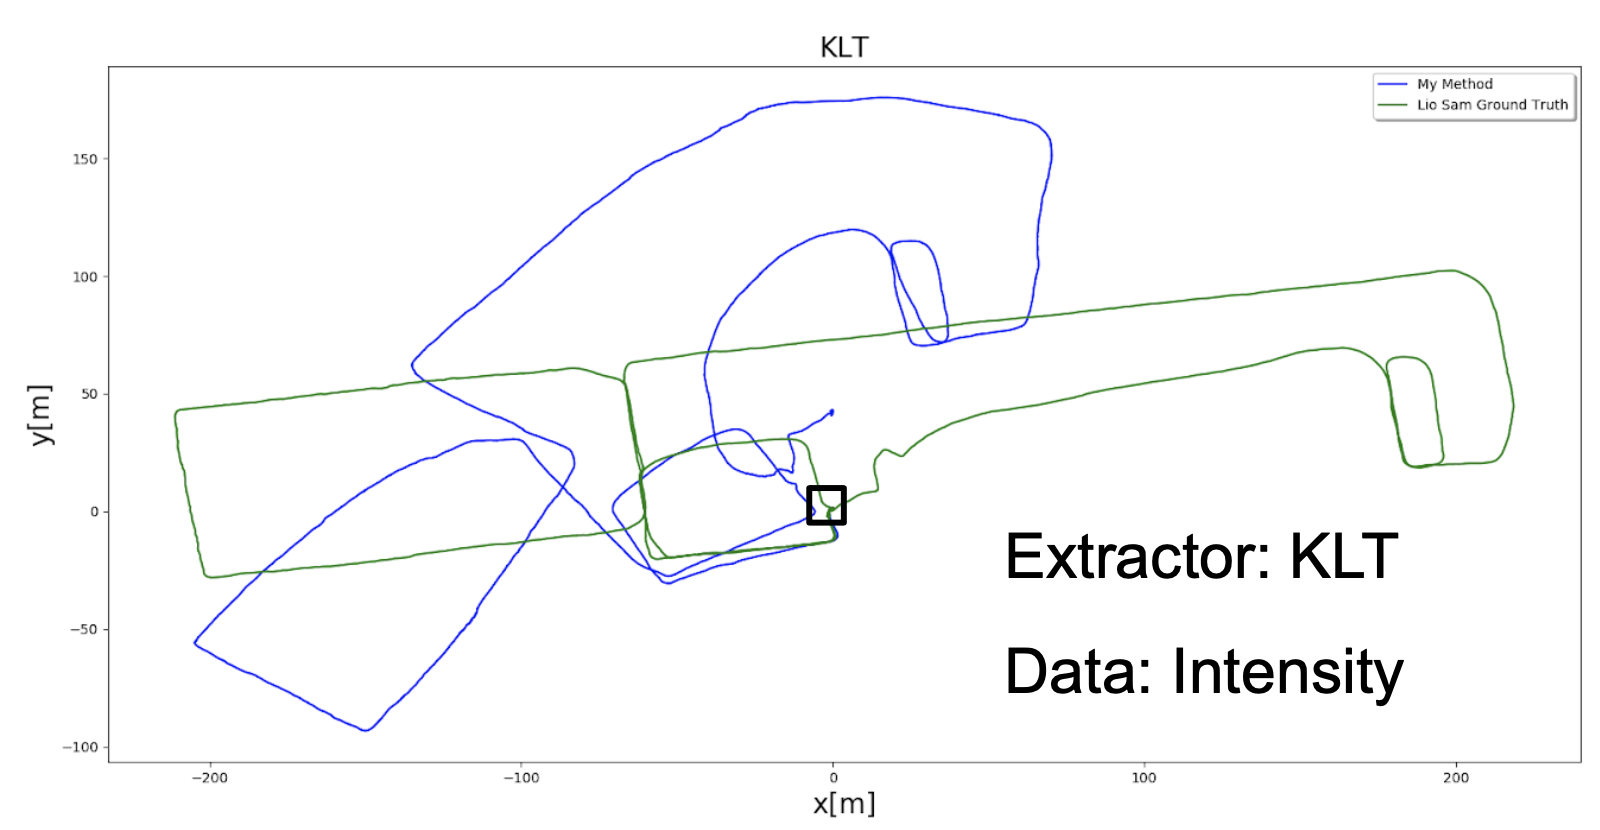
\includegraphics[scale = 0.45]{images/results/mm_trajectory.png}
%             \caption{This works methods trajectory}
%             \label{fig:mm_trajectory}
%         \end{figure}

%         When looking at method from this paper it does accumulate quite some drift but performs considerably better than the scan based LOAM implementation. For additional performance results of this method consult \cref{sec:additional_results}
%     }
%     \clearpage
% }

    
% \section{Final Comparison of Feature Methods}{
%         In this section I will perform a comparison of the feature methods to the point of a possible verdict. For in depth data about each respective method consult \cref{ch:additional_plots}

%         \subsection{Local Step Comparison – feature methods}{

%         \begin{tabular}{p{2cm} p{3.5cm} p{3.7cm} p{2cm}}
%             & \textbf{ORB} & \textbf{BRISK} & \textbf{KLT}
%         \end{tabular}

%         \begin{table}[!ht]
%             \setlength{\extrarowheight}{5pt}
%             \centering
%             \large
%             \begin{tabular}{p{1.3cm}| p{1.5cm} p{1.5cm}| p{1.5cm} p{1.5cm}| p{1.5cm} p{1.5cm}}
%                 \hline
%                 \textbf{Errors} & Mean & STD & Mean & STD & Mean & STD\\[12pt]
%                 \hline
%                 X[m] & -0.004 & 0.056 & 0.004 & 0.219 & \text{\color{Green}{-0.003}} & \text{\color{Cyan}{0.048}}\\[3pt]
%                 \hline
%                 Y[m] & \text{\color{Green}{0}} & 0.040 & \text{\color{Green}{0}} & 0.117 & 0.001 & \text{\color{Cyan}{0.035}}\\[3pt]
%                 \hline
%                 Z[m] & -0.001 & 0.058 & -0.001 & 0.097 & \text{\color{Green}{0}} & \text{\color{Cyan}{0.046}}\\[3pt]
%                 \hline
%                 Roll[°] & \text{\color{Green}{0}} & \text{\color{Cyan}{0.024}} & 0.001 & 0.049 & \text{\color{Green}{0}} & 0.025\\[3pt]
%                 \hline
%                 Pitch[°] & \text{\color{Green}{0}} & \text{\color{Cyan}{0.024}} & \text{\color{Green}{0}} & 0.028 & \text{\color{Green}{0}} & \text{\color{Cyan}{0.024}}\\[3pt]
%                 \hline
%                 Yaw[°] & \text{\color{Green}{0}} & \text{\color{Cyan}{0.024}} & \text{\color{Green}{0}} & 0.048 & \text{\color{Green}{0}} & 0.029\\[3pt]
%             \end{tabular}
%             \caption{Average Step Error Comparison for Feature Methods}
%             \label{tab:step_errors_methods}
%         \end{table}

%         In \cref{tab:step_errors_methods} we can see the iterative performance of the feature methods. 
        
%         ORB and KLT seem to perform similarly while BRISK falls off a little regarding the standard deviation.

%         }
%         \subsection{Trajectory Comparison – feature methods}{

%         \begin{figure}[!ht]
%             \centering
%             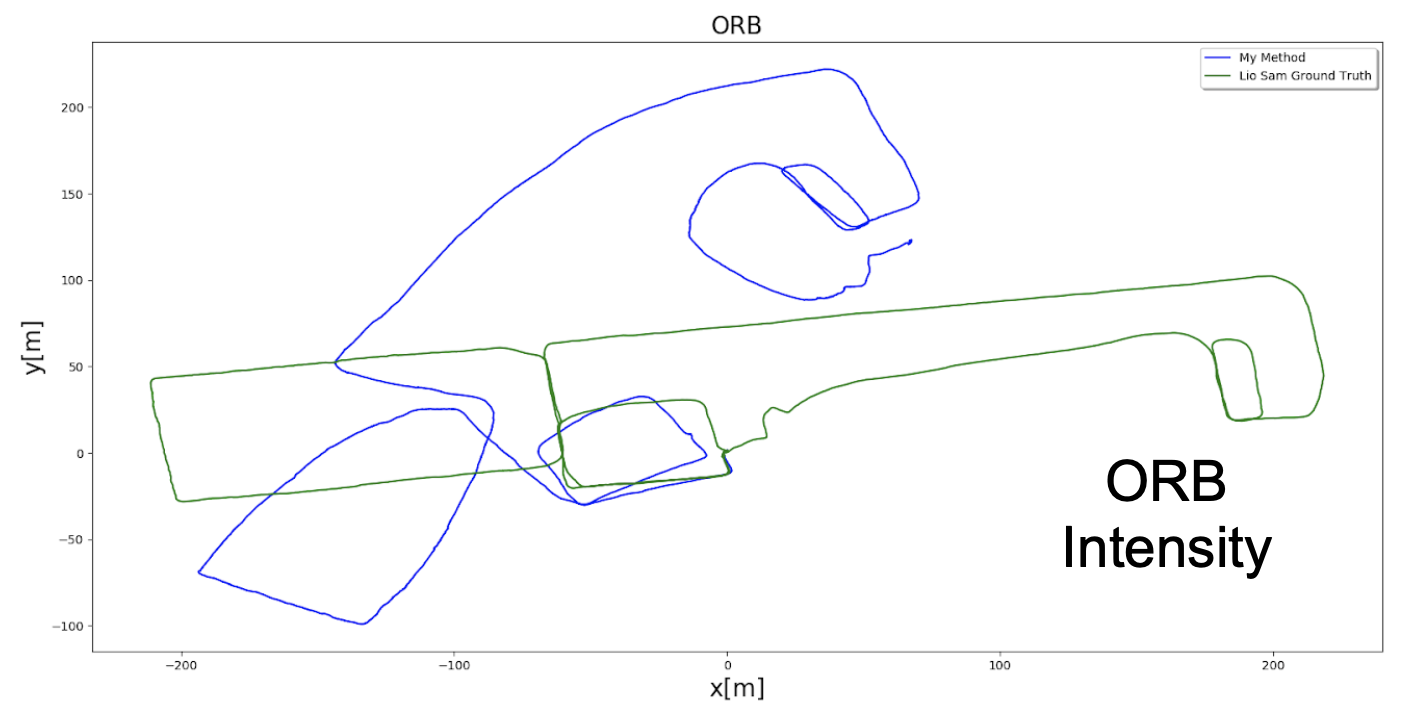
\includegraphics[scale = 0.5]{images/comparison_appendix/ORBt.png}
%             \caption{ORB trajectory}
%             \label{fig:ORB_trajectory}
%         \end{figure}
%         \clearpage

%         \begin{figure}[!ht]
%             \centering
%             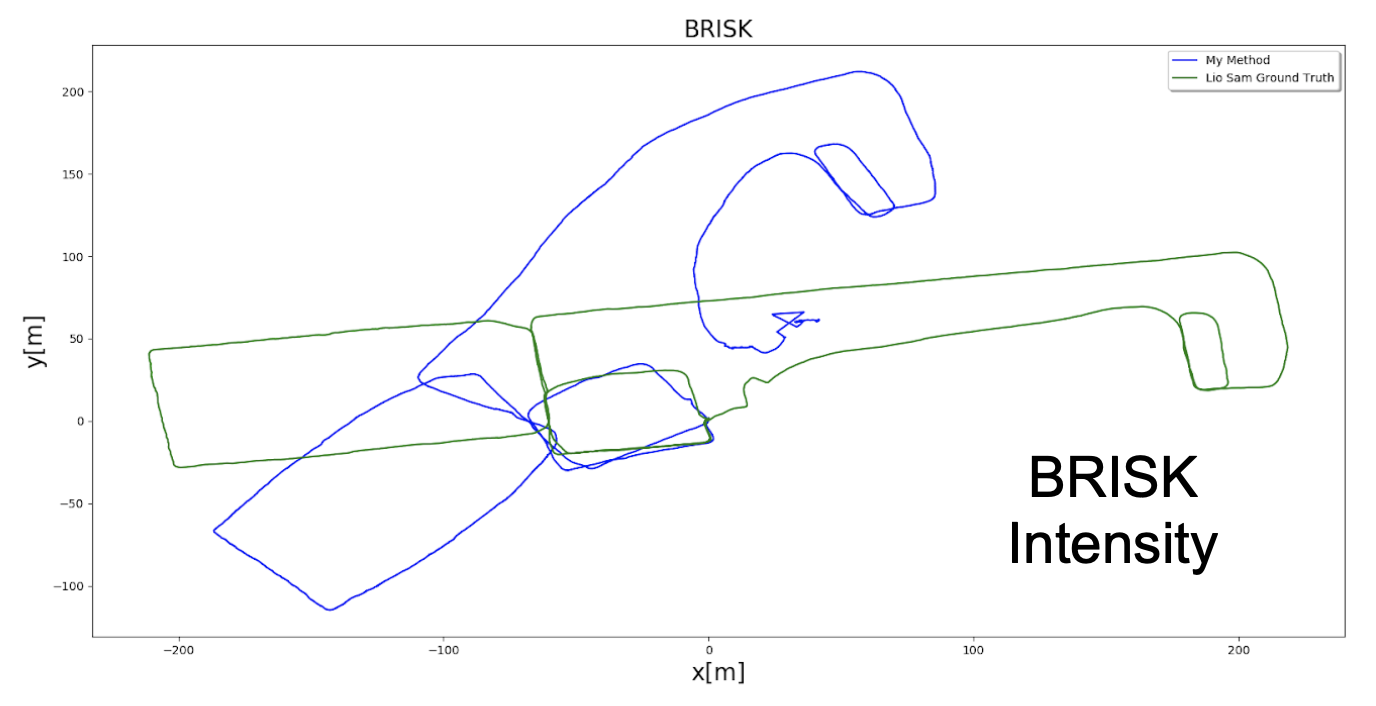
\includegraphics[scale = 0.5]{images/comparison_appendix/BRISKt.png}
%             \caption{BRISK trajectory}
%             \label{fig:BRISK_trajectory}
%         \end{figure}

%         \begin{figure}[!ht]
%             \centering
%             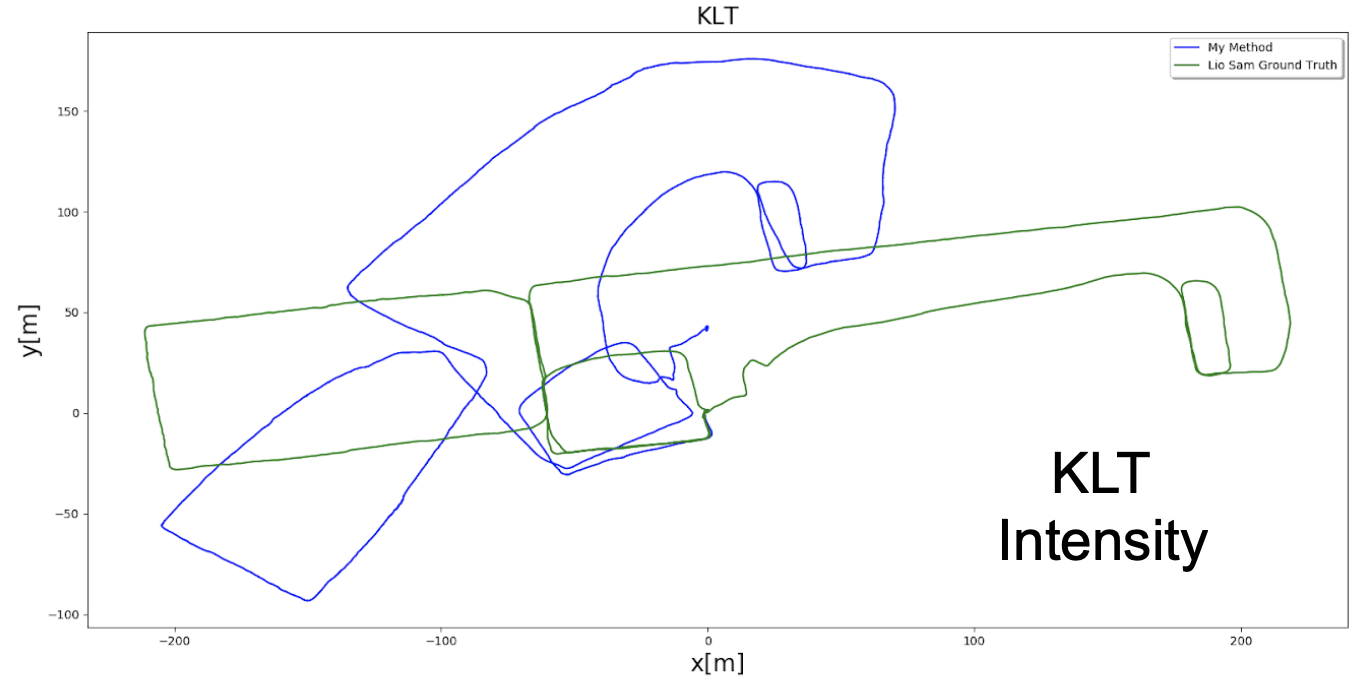
\includegraphics[scale = 0.5]{images/comparison_appendix/KLTt.png}
%             \caption{KLT trajectory}
%             \label{fig:KLT_trajectory_method}
%         \end{figure}
%         }
%         \clearpage
%         \subsection{Drift Comparison – feature methods}{
%             I also compared the more promising methods ORB and KLT regarding the accumulated drift:
%             \subsubsection{Translational Drift - feature methods}{
%                 \begin{figure}[!ht]
%                     \centering
%                     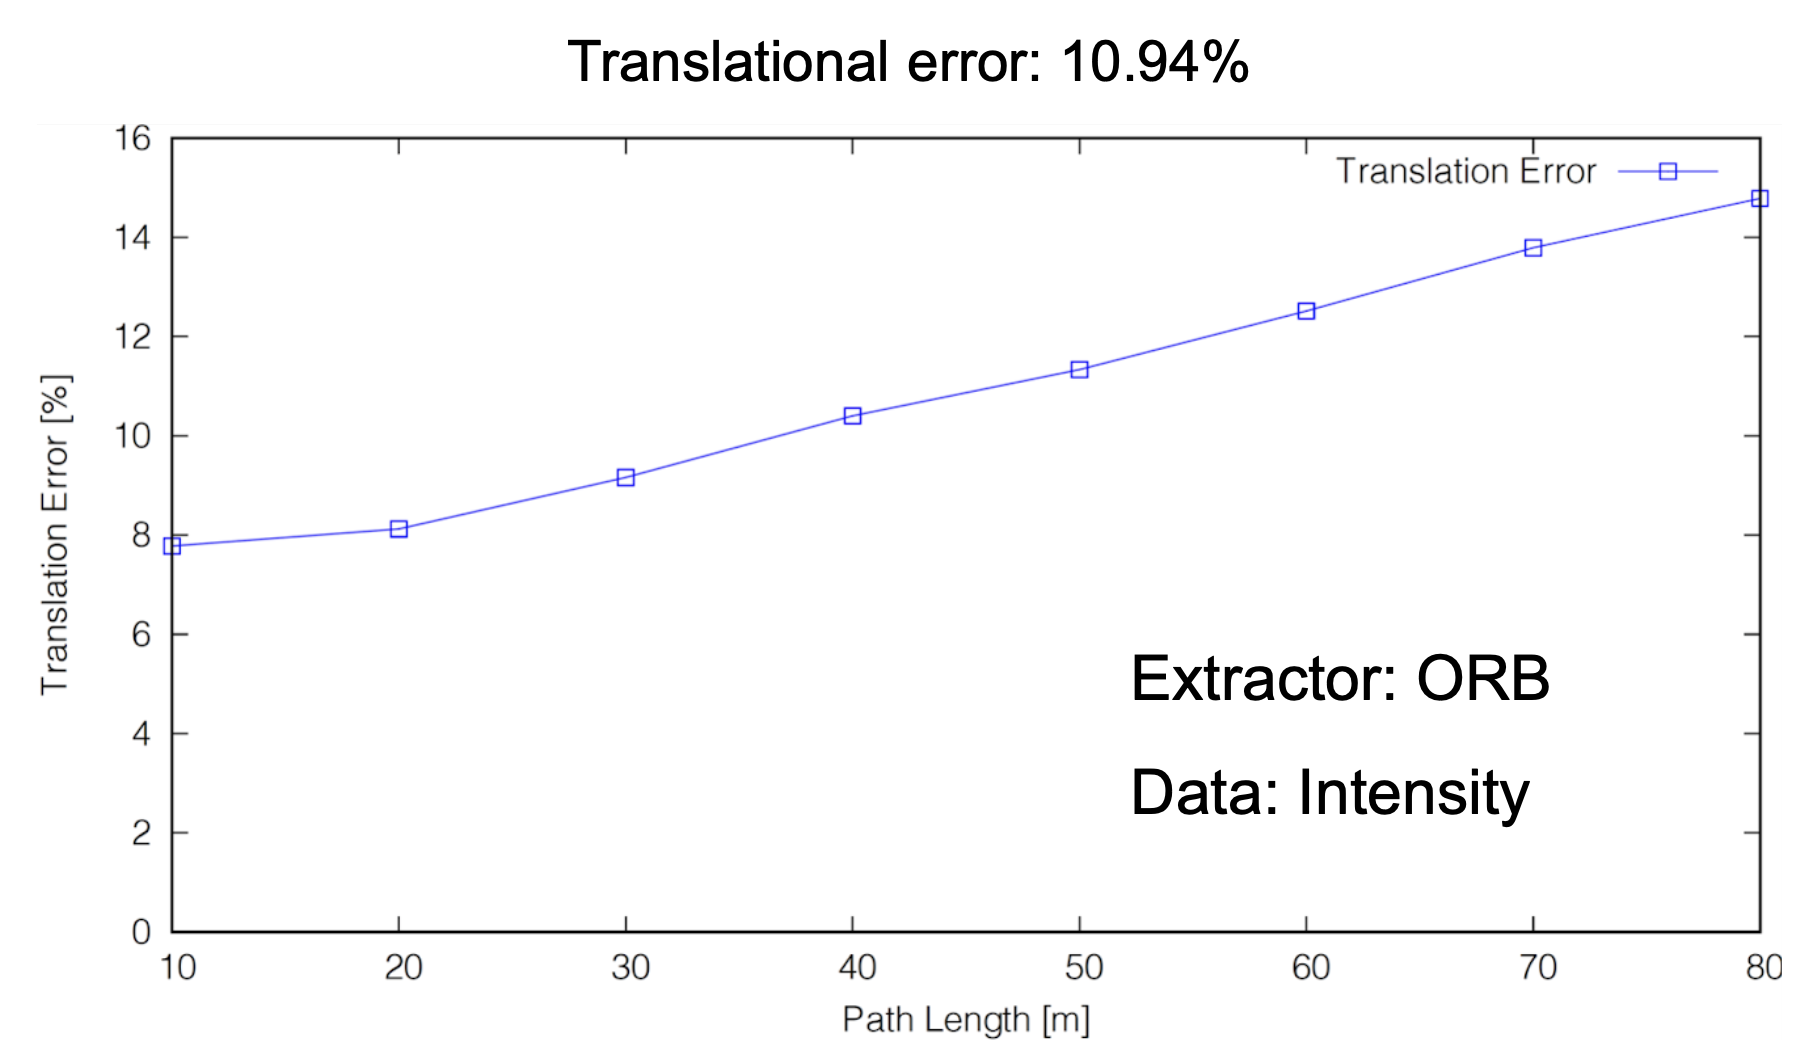
\includegraphics[scale = 0.4]{images/comparison_appendix/orb_drift_transl.png}
%                     \caption{ORB drift translation}
%                     \label{fig:ORB_drift_transl}
%                 \end{figure}

%                 \begin{figure}[!ht]
%                     \centering
%                     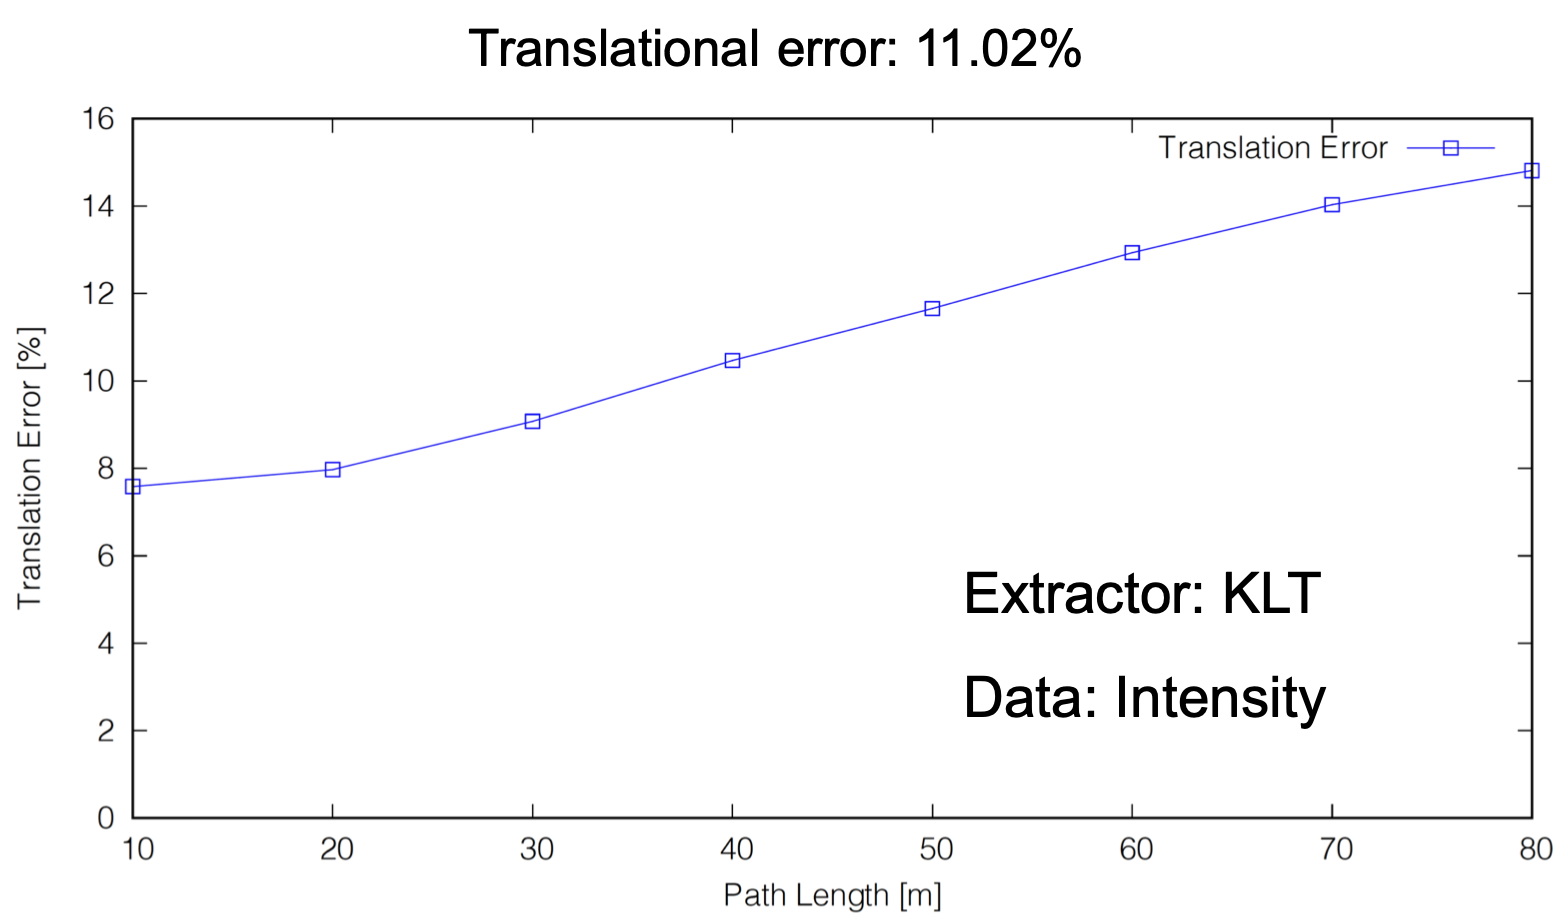
\includegraphics[scale = 0.45]{images/results/mm_drift_translation.png}
%                     \caption{KLT translational drift}
%                     \label{fig:KLT_drift_transl}
%                 \end{figure}
%                     }
%                 \clearpage
%             \subsubsection{Angular Drift - feature methods}{

%                 \begin{figure}[!ht]
%                     \centering
%                     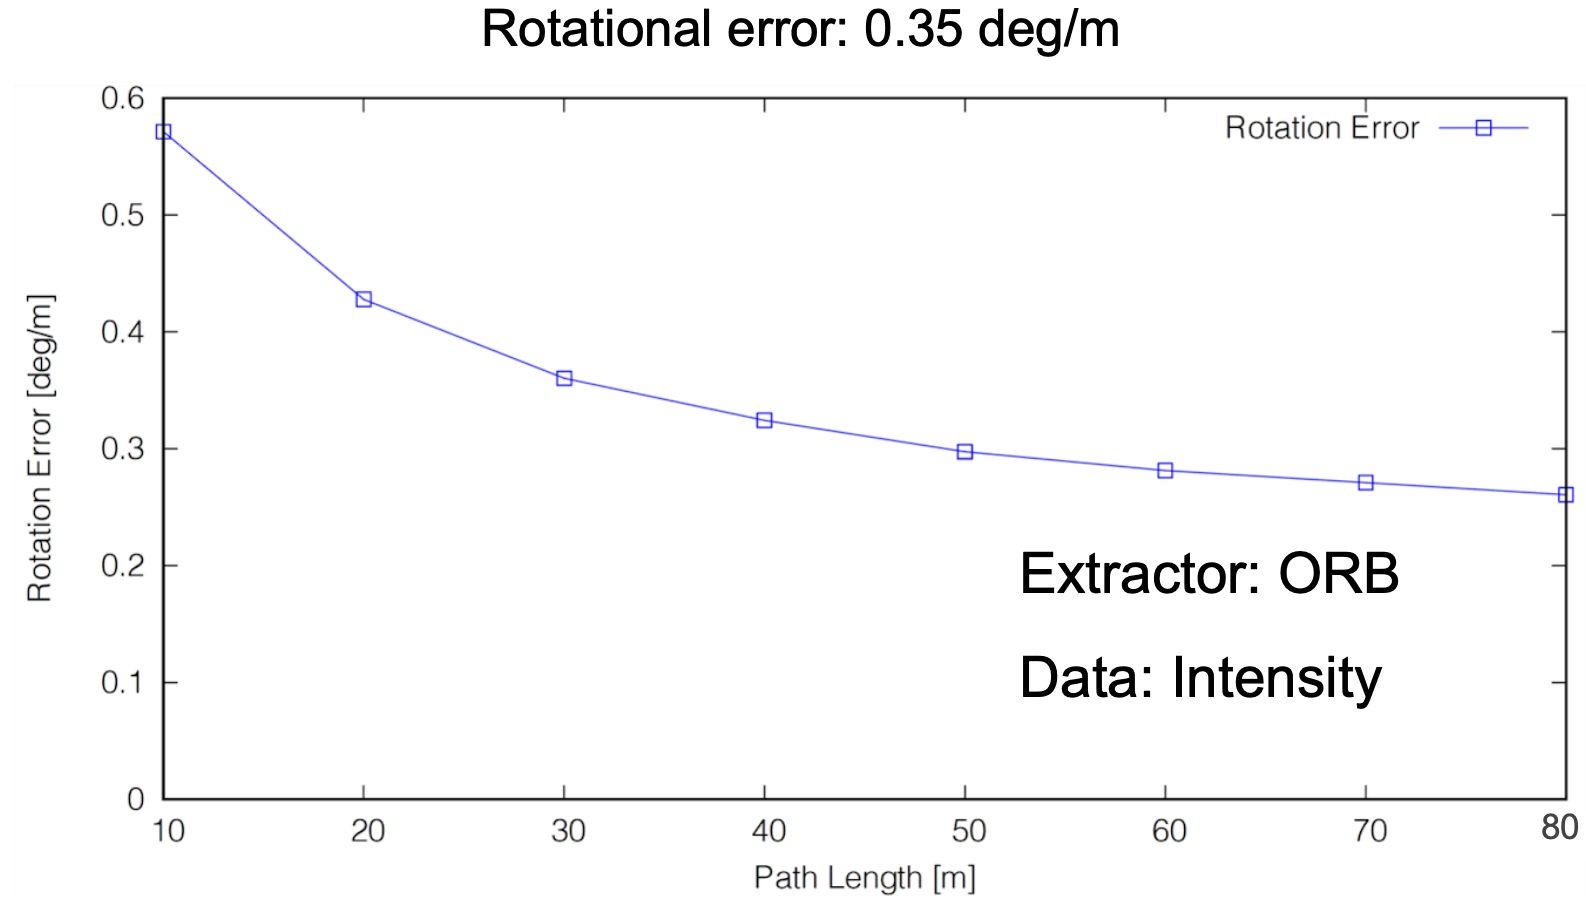
\includegraphics[scale = 0.45]{images/comparison_appendix/orb_drift_angle.png}
%                     \caption{ORB angular drift}
%                     \label{fig:ORB_drift_angle}
%                 \end{figure}

%                 \begin{figure}[!ht]
%                     \centering
%                     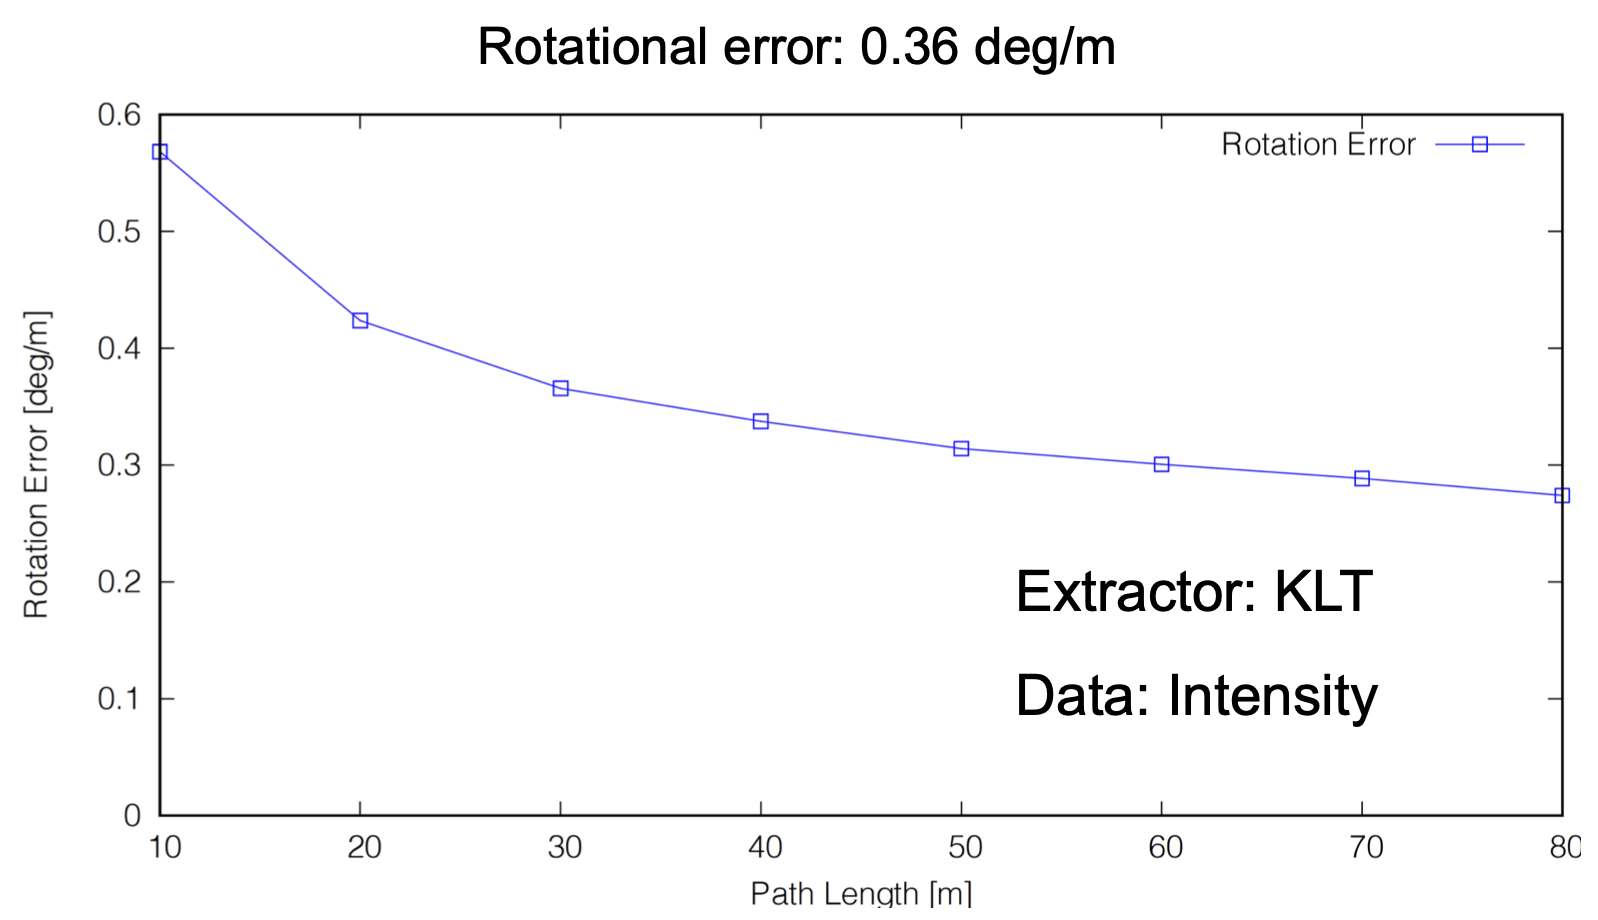
\includegraphics[scale = 0.45]{images/results/mm_drift_angle.png}
%                     \caption{KLT angular drift}
%                     \label{fig:KLT_drift_angle}
%                 \end{figure}
%             }
%             As we can see on the drift plots \cref{fig:ORB_drift_transl} to \cref{fig:KLT_drift_angle} ORB performs slightly better than KLT for the considered dataset.
                    
%         }
%         \clearpage
%         \subsection{Verdict Feature Methods}{

%             Starting of with the step comparison ORB and KLT indicate a slightly better performance than BRISK. 

%             With the additional consideration of BRISKs comparatively poor TP rate and higher computational cost I would chose ORB or KLT over BRISK for the endeavor pursued in this work.

%             Then for the comparison of ORB and KLT we can see that ORB performs a little bit better considering the global drift error. However we have to consider the fundamental difference in their procedure. While ORB is dependent on the extraction of points at each iteration KLT can make use of previously detected points. This can be an advantage especially in feature-scarce environments. This is shown well in the additinal performance results section \cref{sec:additional_results}. So for a final verdict in this comparison I would use ORB on feature rich environments while KLT is more consistent in repetitive and feature scarce surroundings.
%             \clearpage
%         }

        
%     }
    
% \section{Final Comparison of Complementary Data}{

%     \subsection{Local Step Comparison – projection types}{

%     \begin{tabular}{p{2cm} p{3.5cm} p{3.5cm} p{2cm}}
%         \textbf{Errors} & \textbf{Intensity} & \textbf{Ambient} & \textbf{Range}
%     \end{tabular}

%     \begin{table}[!ht]
%         \setlength{\extrarowheight}{5pt}
%         \centering
%         \large
%         \begin{tabular}{p{1.3cm}| p{1.5cm} p{1.5cm}| p{1.5cm} p{1.5cm}| p{1.5cm} p{1.5cm}}
%             \hline
%                 & Mean & STD & Mean & STD & Mean & STD\\[12pt]
%             \hline
%             X[m] & -0.004 & \text{\color{Cyan}{0.056}} & -0.007 & 0.060 & \text{\color{Green}{-0.002}} & 0.102\\[3pt]
%             \hline
%             Y[m] & \text{\color{Green}{0}} & \text{\color{Cyan}{0.040}} & -0.001 & 0.042 & -0.008 & 0.170\\[3pt]
%             \hline
%             Z[m] & -0.001 & \text{\color{Cyan}{0.058}} & \text{\color{Green}{0}} & 0.060 & \text{\color{Green}{0}} & 0.098\\[3pt]
%             \hline
%             Roll[°] & \text{\color{Green}{0}} & \text{\color{Cyan}{0.024}} & \text{\color{Green}{0}} & \text{\color{Cyan}{0.024}} & 0.001 & 0.072\\[3pt]
%             \hline
%             Pitch[°] & \text{\color{Green}{0}} & \text{\color{Cyan}{0.024}} & \text{\color{Green}{0}} & \text{\color{Cyan}{0.024}} & \text{\color{Green}{0}} & 0.039\\[3pt]
%             \hline
%             Yaw[°] & \text{\color{Green}{0}} & \text{\color{Cyan}{0.029}} & \text{\color{Green}{0}} & \text{\color{Cyan}{0.029}} & \text{\color{Green}{0}} & 0.040\\[3pt]
%         \end{tabular}
%         \caption{Average Step Error Comparison for Complementary Data}
%         \label{tab:step_errors_data}
%     \end{table}

%     In \cref{tab:step_errors_data} intensity performs best directly followed best by the ambient data. Range falls off considering the standard deviation.
%     }

    
    
%     \subsection{Trajectory Comparison – projection types}{

%         \begin{figure}[!ht]
%             \centering
%             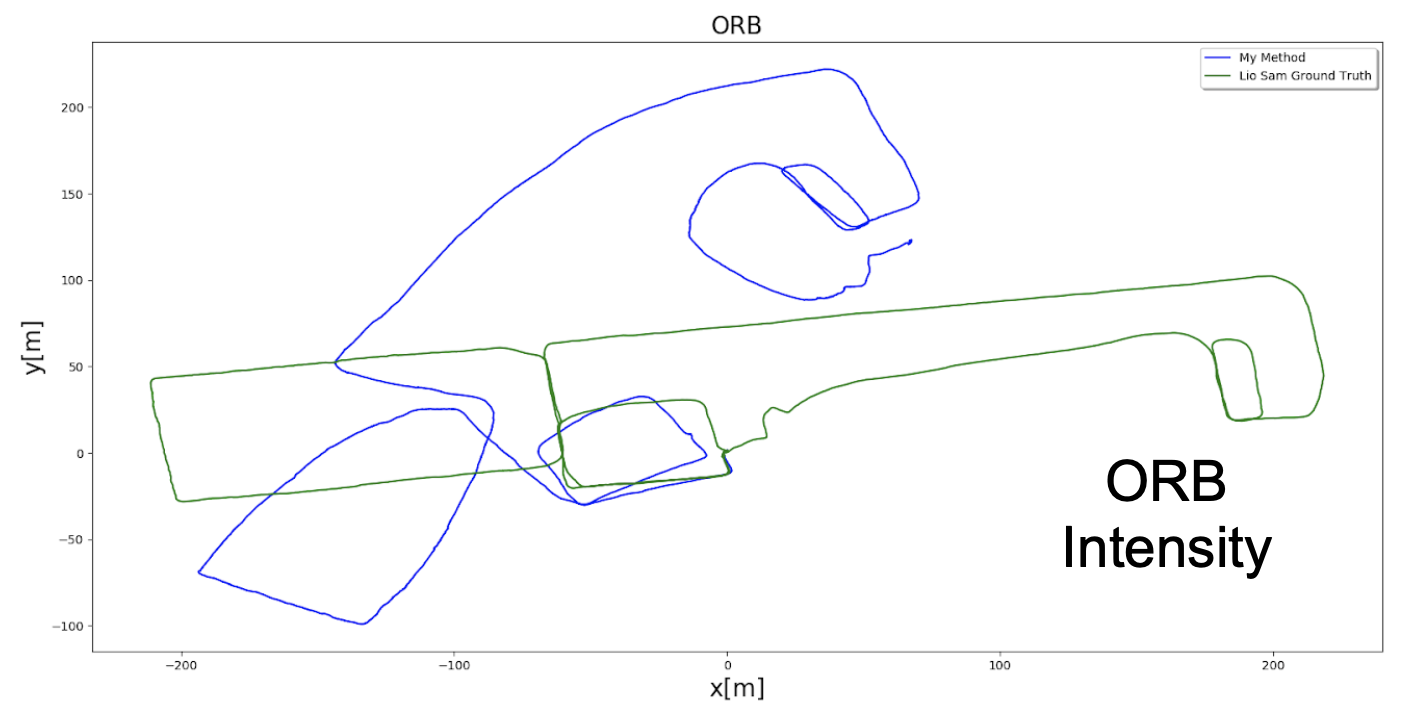
\includegraphics[scale = 0.5]{images/comparison_appendix/ORBt.png}
%             \caption{ORB trajectory}
%             \label{fig:ORB_trajectory_data}
%         \end{figure}
%         \clearpage

%         \begin{figure}[!ht]
%             \centering
%             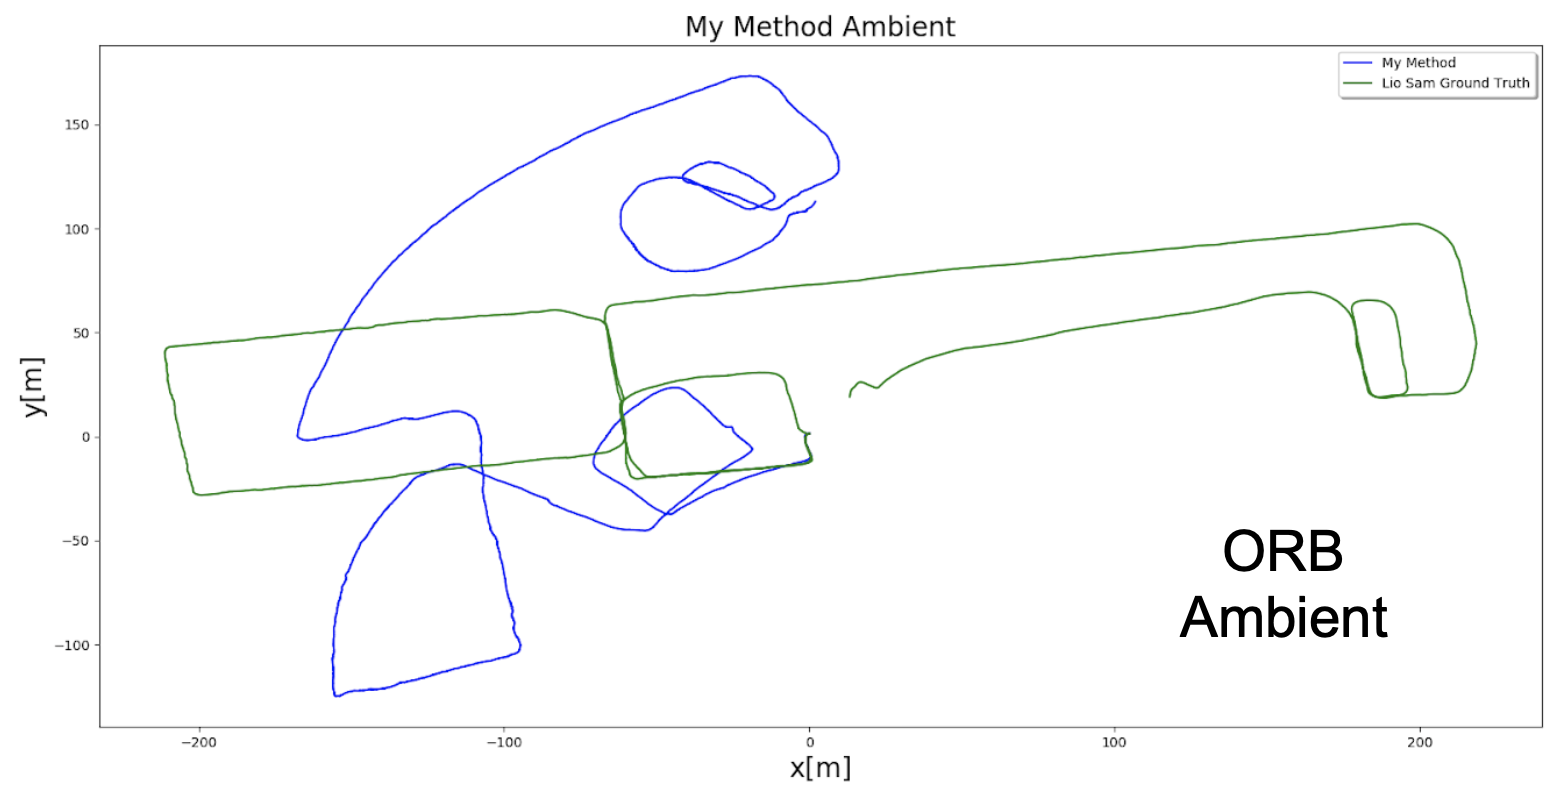
\includegraphics[scale = 0.5]{images/comparison_appendix/Ambientt.png}
%             \caption{Ambient trajectory}
%             \label{fig:ambient_trajectory}
%         \end{figure}

%         \begin{figure}[!ht]
%             \centering
%             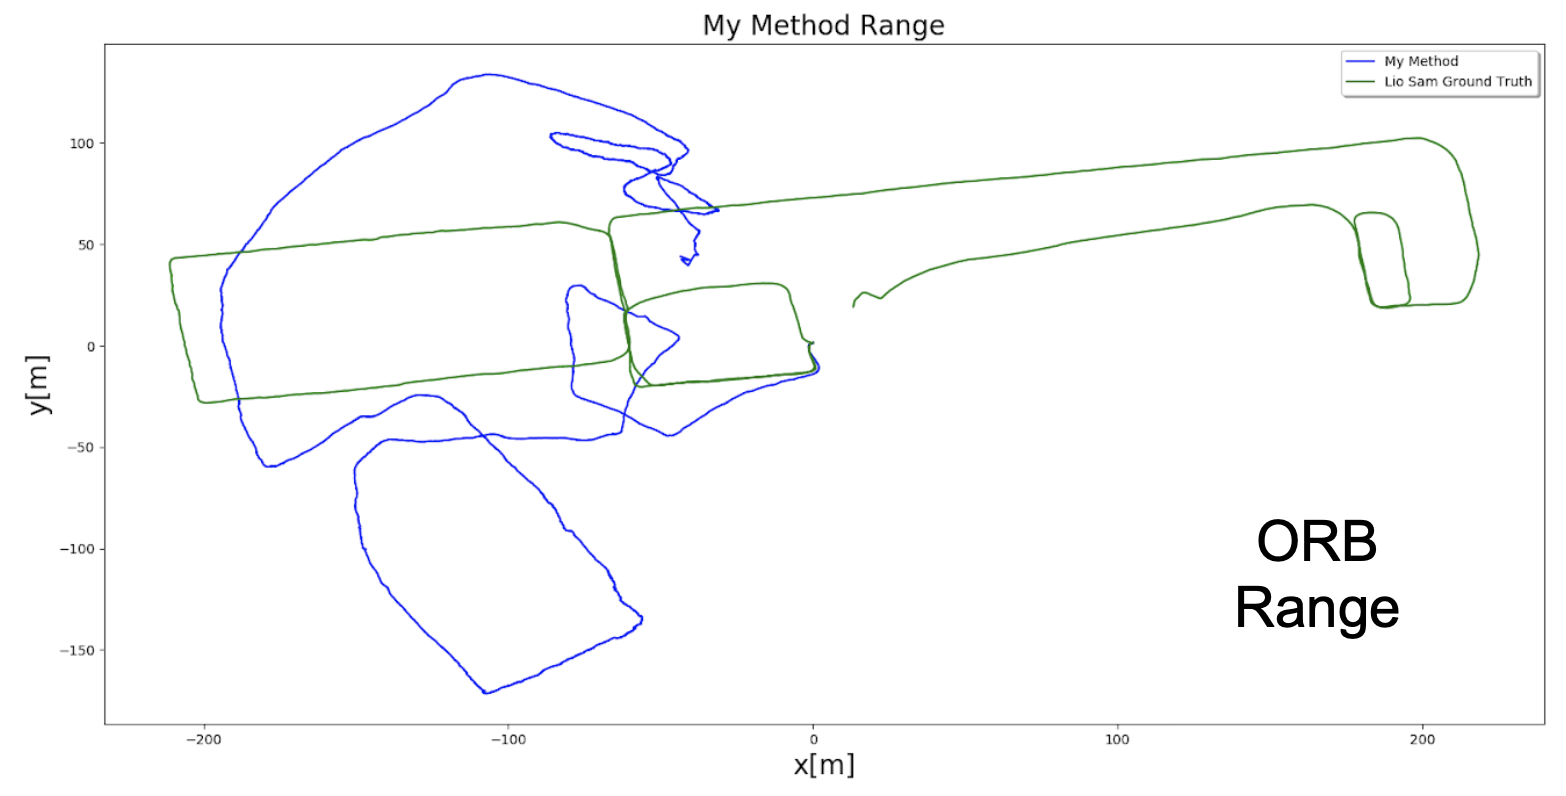
\includegraphics[scale = 0.5]{images/comparison_appendix/Ranget.png}
%             \caption{Range trajectory}
%             \label{fig:range_trajectory_method}
%         \end{figure}

%     }
%     \clearpage

%     \subsection{Drift Comparison – projection types}{
%         Analogously the accumulated drift comparison for the two more promising data types intensity and ambient:
%         \subsubsection{Translational Drift - projection types}{
%             \begin{figure}[!ht]
%                 \centering
%                 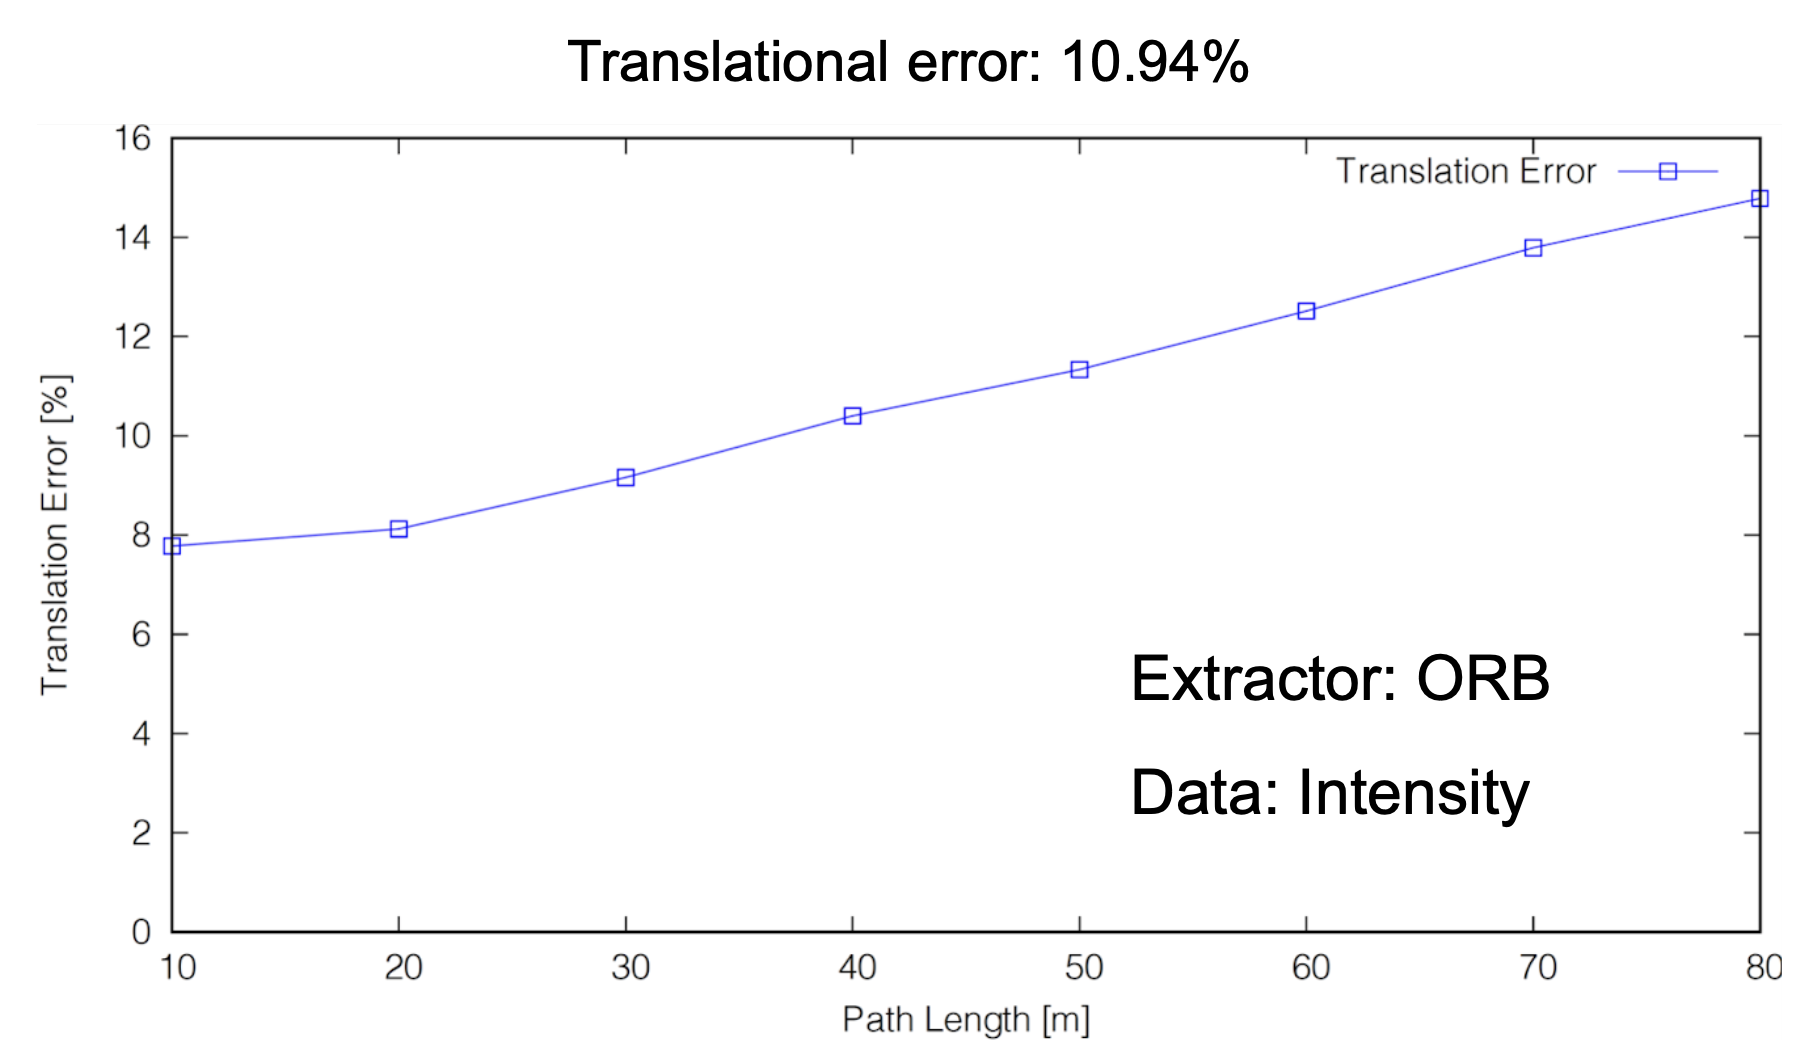
\includegraphics[scale = 0.4]{images/comparison_appendix/orb_drift_transl.png}
%                 \caption{Intensity drift translation}
%                 \label{fig:intensity_drift_transl}
%             \end{figure}

%             \begin{figure}[!ht]
%                 \centering
%                 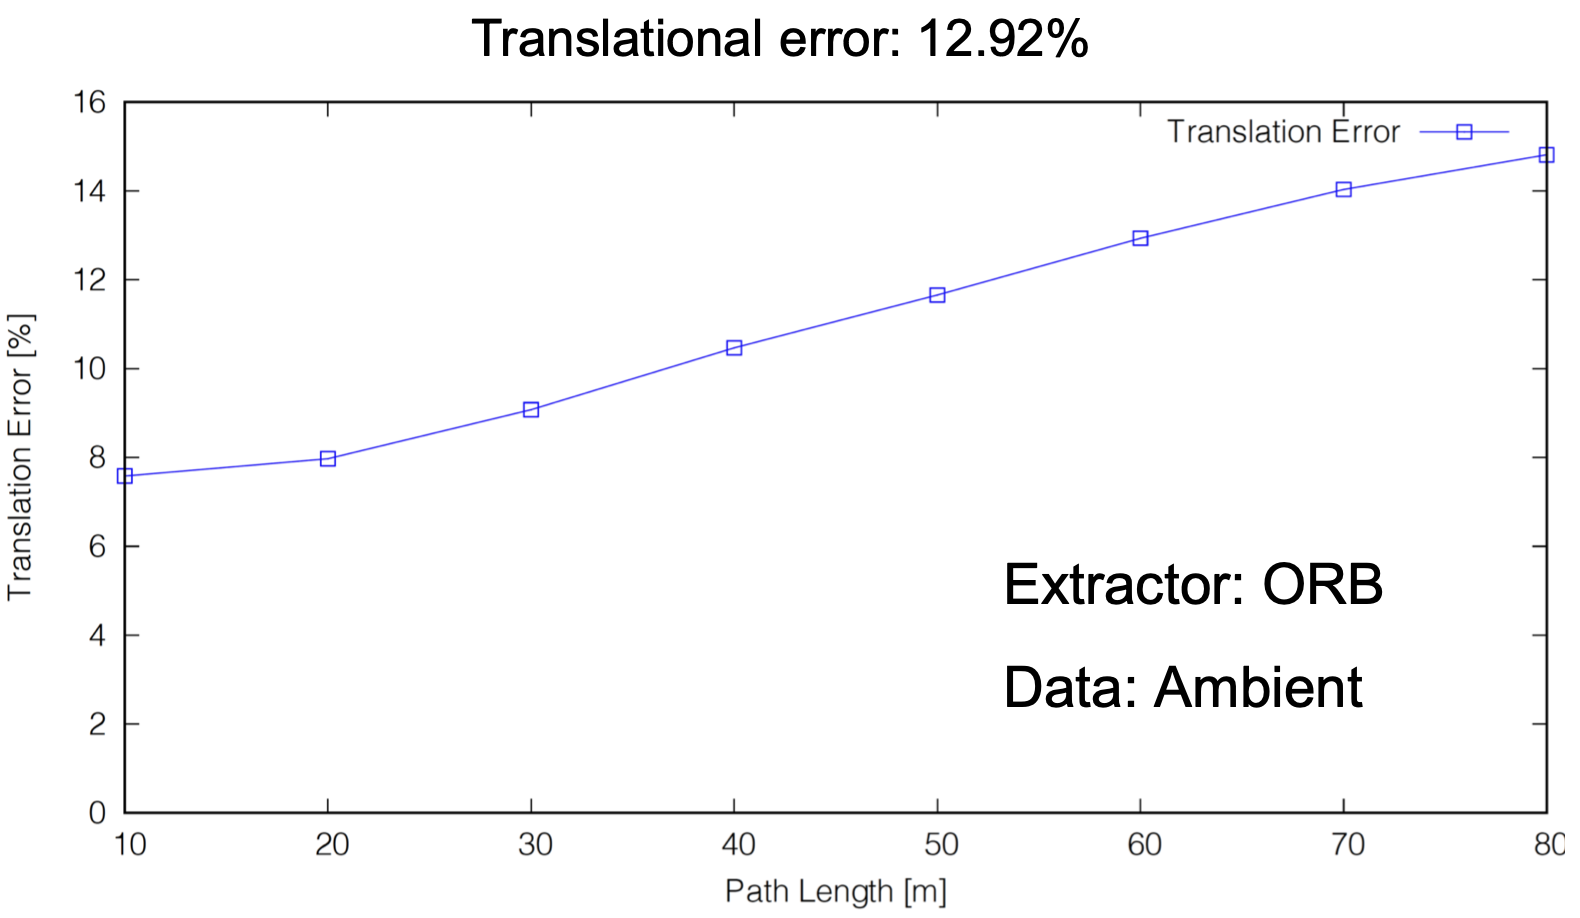
\includegraphics[scale = 0.45]{images/comparison_appendix/ambient_drift_translation.png}
%                 \caption{Ambient drift translation}
%                 \label{fig:ambient_drift_transl}
%             \end{figure}

%         }
%         \clearpage
%         \subsubsection{Angular Drift - projection types}{
%             \begin{figure}[!ht]
%                 \centering
%                 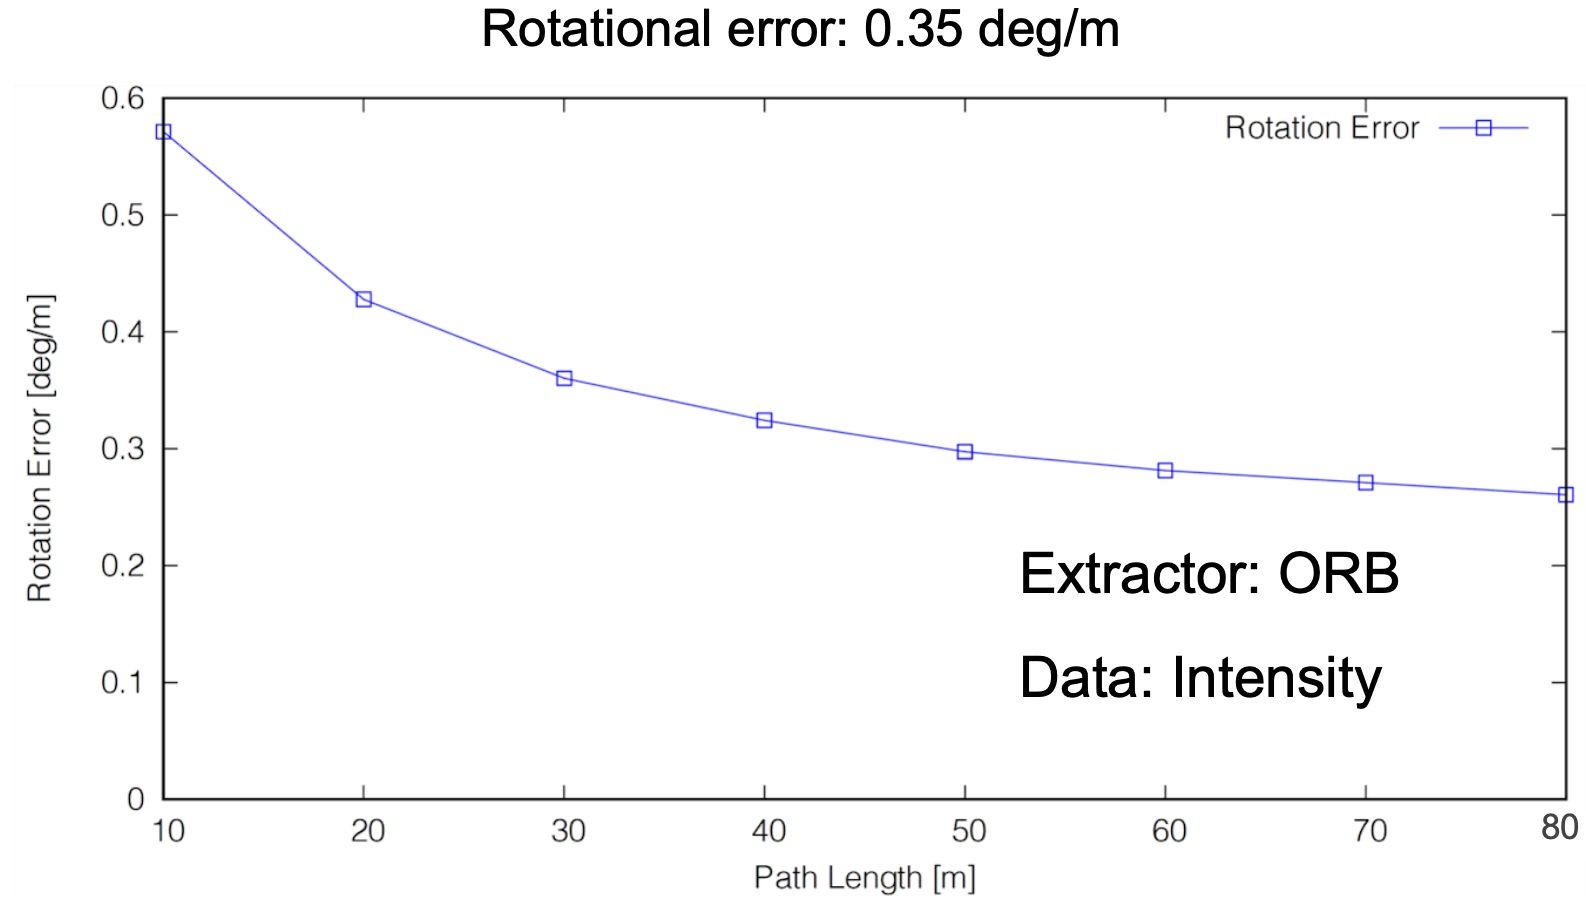
\includegraphics[scale = 0.43]{images/comparison_appendix/orb_drift_angle.png}
%                 \caption{Intensity angular drift}
%                 \label{fig:intensity_drift_angle}
%             \end{figure}

%             \begin{figure}[!ht]
%                 \centering
%                 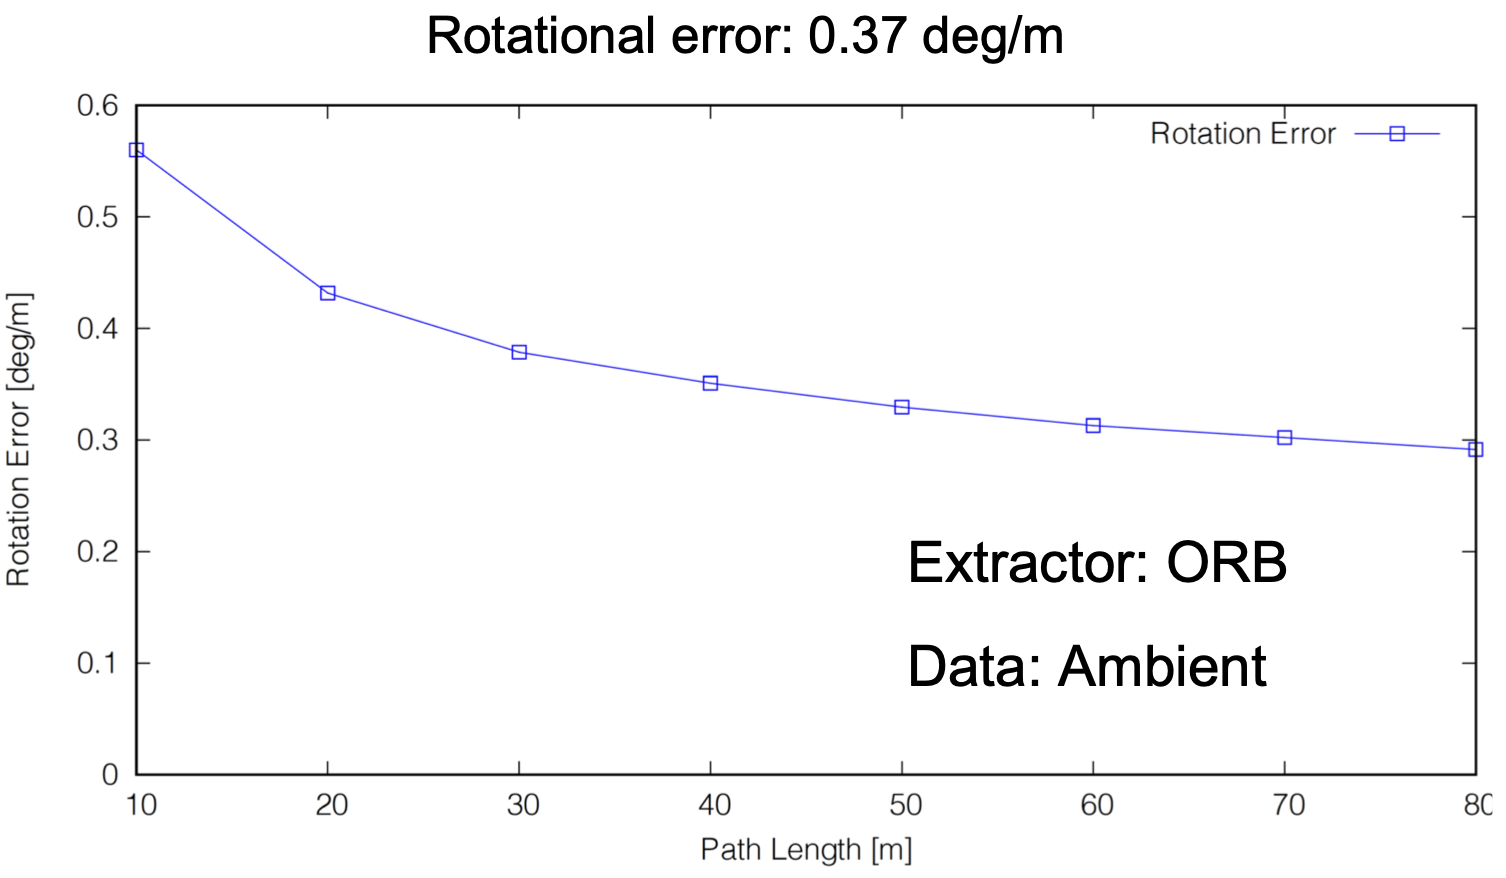
\includegraphics[scale = 0.45]{images/comparison_appendix/ambient_drift_angle.png}
%                 \caption{Ambient angular drift}
%                 \label{fig:ambient_drift_angle}
%             \end{figure}

%         }
%         On the drift plots \cref{fig:intensity_drift_transl} to \cref{fig:ambient_drift_angle} we see the intensity data performing better than ambient.
%     }
%     \clearpage
%     \subsection{Verdict Complementary Data}{

%     For this comparison the story is very similar for each stage in the progression. Intensity and ambient data perform equally well as the data source with a small advantage of intensity data. Range however falls off heavily. This can be seen throughout the whole pipeline. Fewer matches were built, a smaller TP rate was detected, bigger iterative as well as global errors could be found and a worse trajectory estimation resulted. 

%     \vspace{0.5cm}
%     The small gap between intensity and ambient data becomes noticeable when considering the laser intensities light independent nature. Therefore my choice for the optimal data source is intensity while keeping the ambient data in mind. Of course a combination of the data sources (and feature methods) considered would be a better solution still but this work revolved exclusively around individual performance comparison.
%     }

% }
% \clearpage

% \section{Additional Performance Results}\label{sec:additional_results}{
%     \subsection{Map Construction using found Transformation}{
%         With the pose estimation and the iterative scans we can build a map as depicted in \cref{fig:local_mapping} and \cref{fig:global_mapping}.
%         \begin{figure}[ht]
%             \centering
%             \includegraphics[scale=0.15]{images/appendix_additionals/map_before.png}
%             \caption{Local mapping performance}
%             \label{fig:local_mapping}
%         \end{figure}
        
%         \begin{figure}[ht]
%             \centering
%             \includegraphics[scale=0.15]{images/appendix_additionals/map_after.png}
%             \caption{Mapping drift after walking one block}
%             \label{fig:global_mapping}
%         \end{figure}

%         As we can see in \cref{fig:local_mapping} locally the estimation is really accurate leading to a detailed map of the surroundings.

%         After having gone around the building block in the dataset however the mapping process shows accumulated drift. (\cref{fig:global_mapping})

%         For a perfect transformation the red-white arrows should be aligned and should lead back to the start position indicated with the black circle.

%     }
%     \clearpage

%     \subsection{Alternative Dataset 1: Indoor}{
%         For a first alternative to the outside dataset I considered an indoor scan from the same paper\citep{robust2021shan} as the handheld dataset. In this dataset three laps are walked through an office space with small corridors. Before the third lap however the LiDAR sensor is turned upside down.

%         \begin{figure}[ht]
%             \centering
%             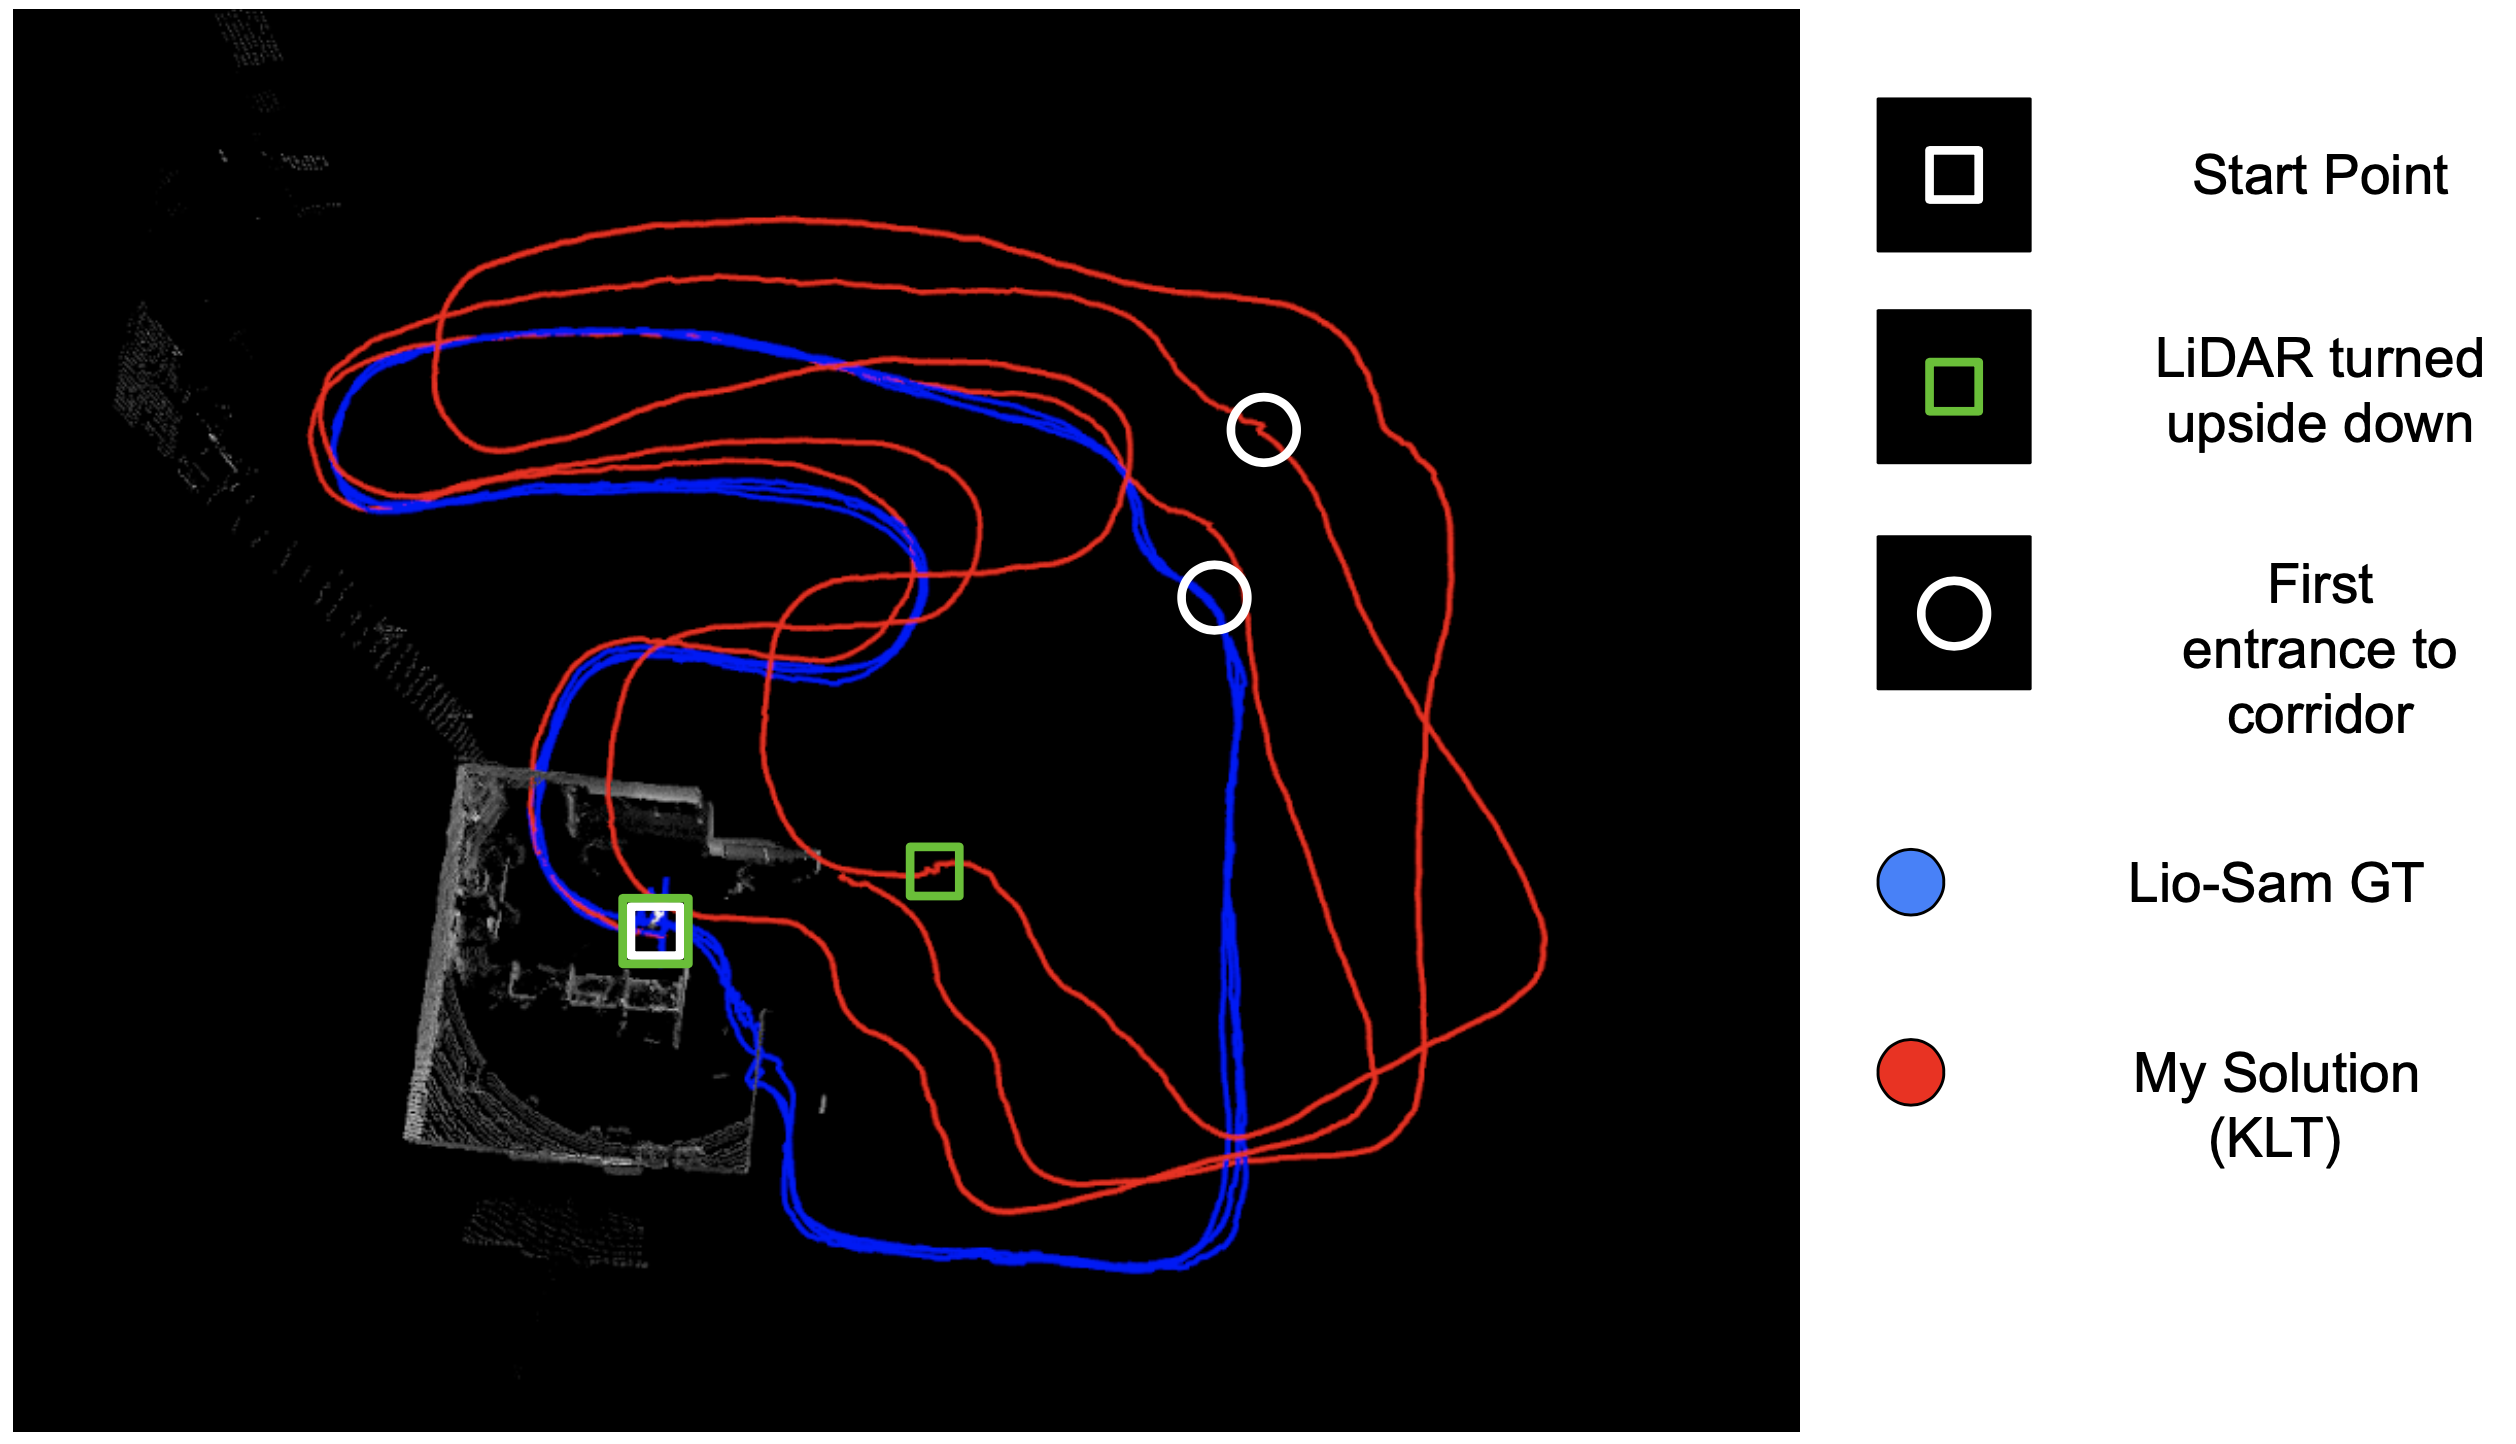
\includegraphics[scale=0.25]{images/appendix_additionals/indoor_klt.png}
%             \caption{Indoor Dataset using KLT}
%             \label{fig:indoor_klt}
%         \end{figure}

%         As we can see there is certain drift accumulating but only slowly. Locally the performance seems quite robust. Also interestingly there is no observable decrease in performance after the second loop. (Sensor turning point)
        
%         This result was achieved using the KLT method. So far ORB and KLT had performed similarly with ORB having slightly smaller errors. Here for this dataset however we have to work with very little features and repetitive surroundings in the corridors. The impact of this can be seen in \cref{fig:indoor_orb} when using ORB:
        
%         \begin{figure}[ht]
%             \centering
%             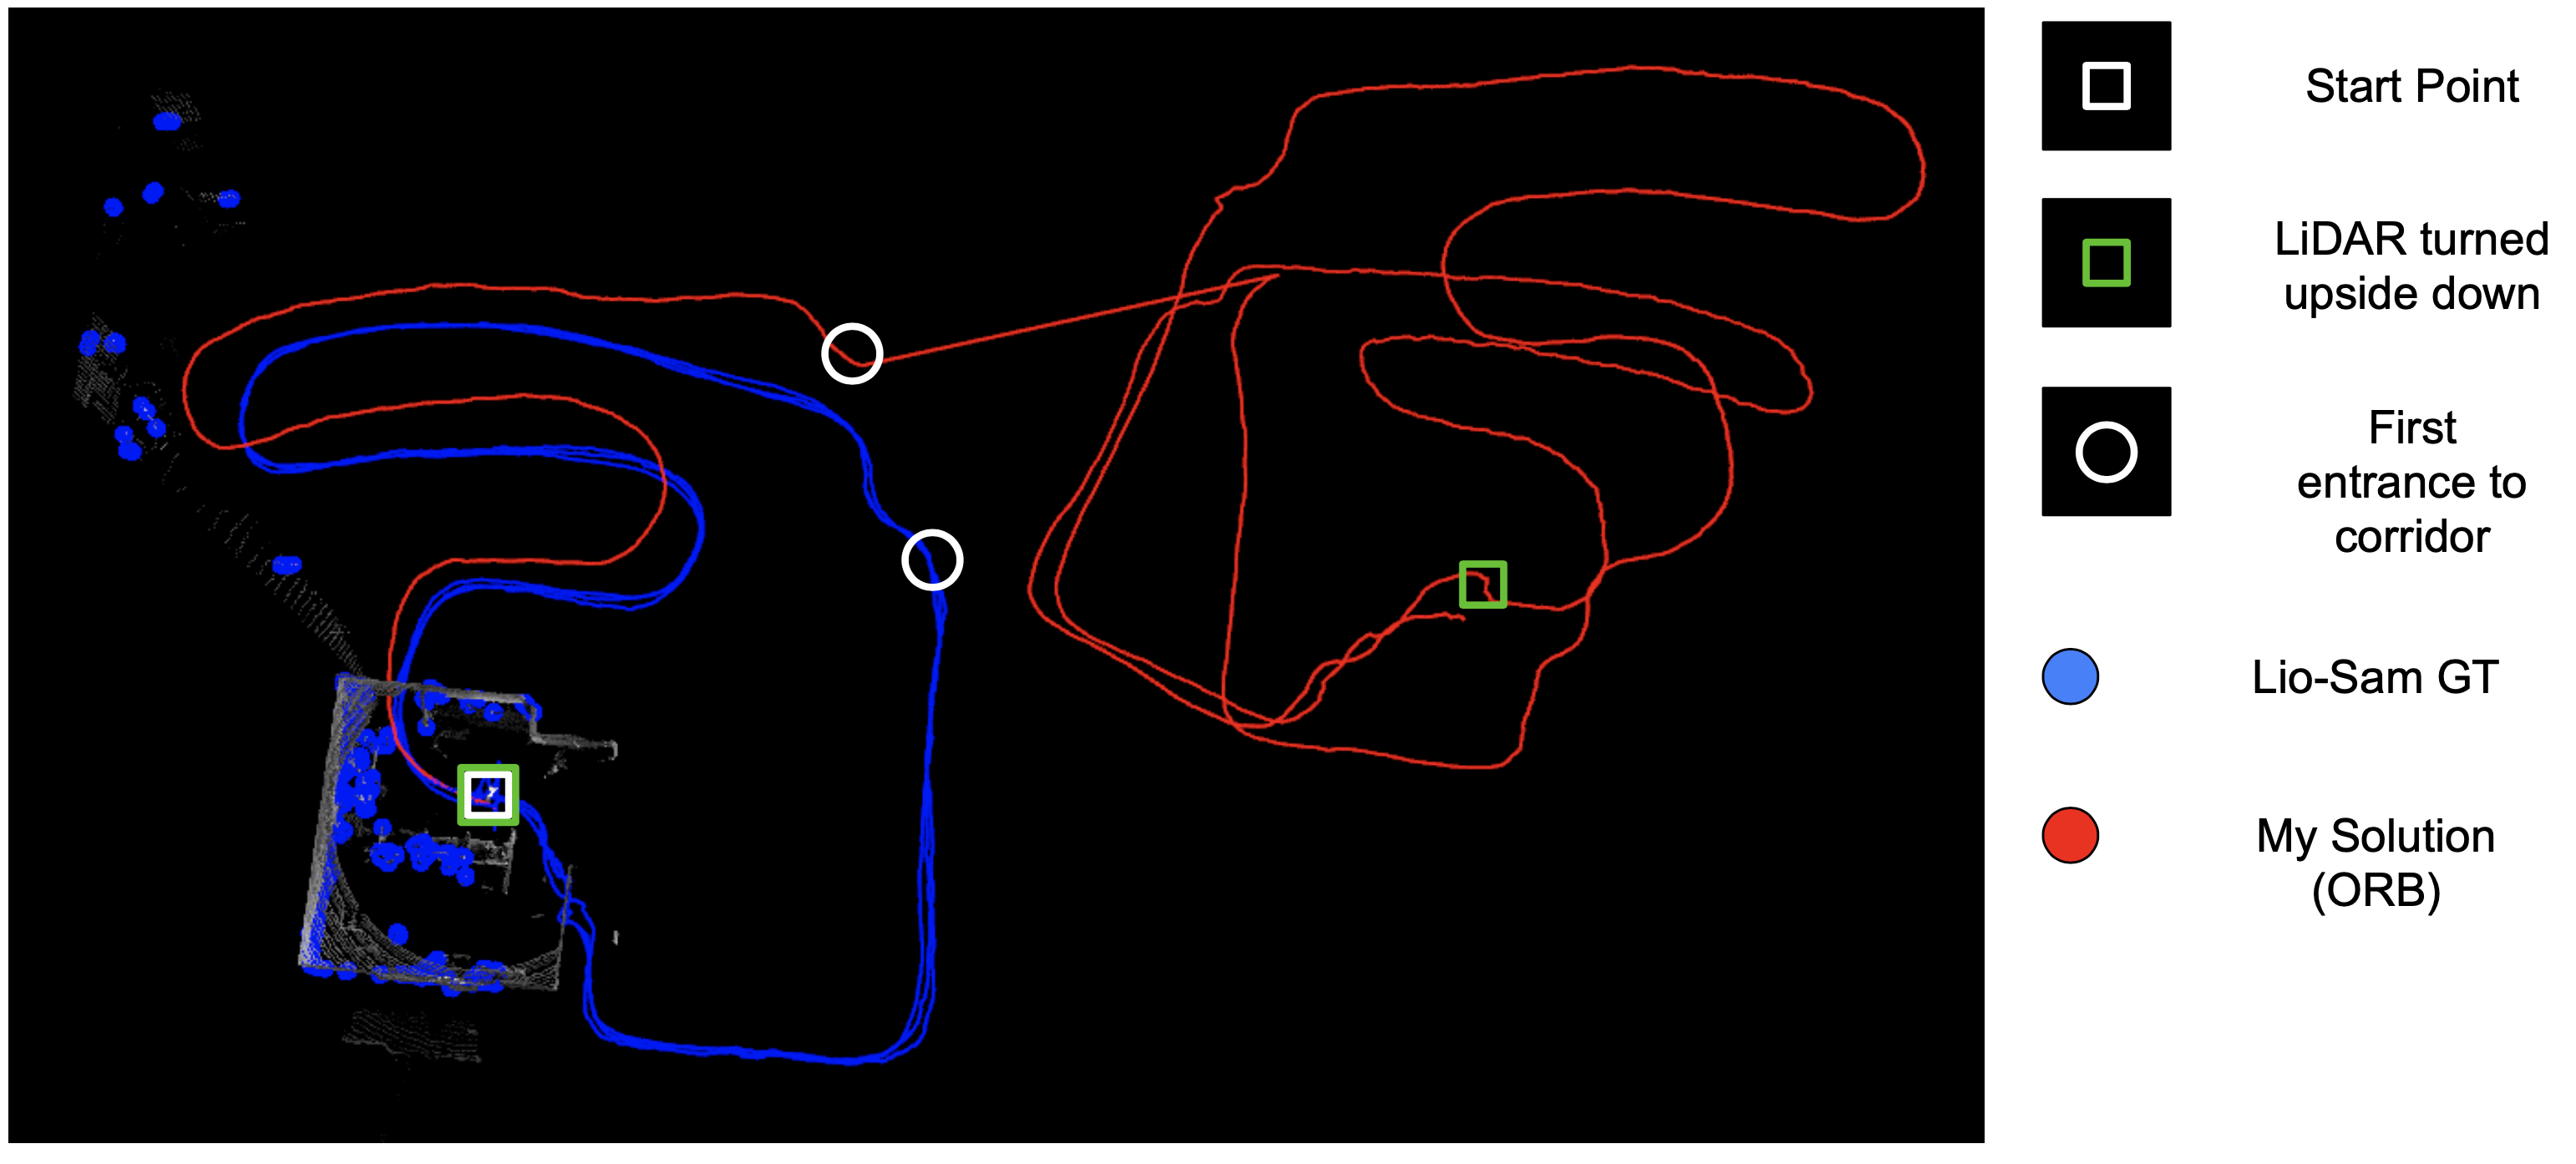
\includegraphics[scale=0.25]{images/appendix_additionals/indoor_orb.png}
%             \caption{Indoor Dataset using ORB}
%             \label{fig:indoor_orb}
%         \end{figure}

%         As we can see ORB performs significantly worse than KLT starting at the entrance point of the corridor (indicated with the white circle) this is of course due to the lack of detectable features while KLT can make use of previously detected key points.

%     }
%     \clearpage

%     \subsection{Alternative Dataset 2: Excavator}{
%     As a second alternative dataset I considered the excavator dataset from the rsl lab.

%     \begin{figure}[ht]
%         \centering
%         \includegraphics[scale=0.15]{images/appendix_additionals/excavator.png}
%         \caption{Map construction on excavator dataset}
%         \label{fig:excavator_map}
%     \end{figure}

%     \normalsize
%     As the name lets assume this dataset is from the point of view of an excavator on a very vast landscape with few features that are located far away. In the lower half of this \cref{fig:excavator_map} we see the map building process analogously to \cref{fig:local_mapping}. Here we see poor performance due to the lack of features and the big distances to them.
% }
% }
